%% abtex2-modelo-trabalho-academico.tex, v-1.9.2 laurocesar
%% Copyright 2012-2014 by abnTeX2 group at http://abntex2.googlecode.com/ 
%%
%% This work may be distributed and/or modified under the
%% conditions of the LaTeX Project Public License, either version 1.3
%% of this license or (at your option) any later version.
%% The latest version of this license is in
%%   http://www.latex-project.org/lppl.txt
%% and version 1.3 or later is part of all distributions of LaTeX
%% version 2005/12/01 or later.
%%
%% This work has the LPPL maintenance status `maintained'.
%% 
%% The Current Maintainer of this work is the abnTeX2 team, led
%% by Lauro César Araujo. Further information are available on 
%% http://abntex2.googlecode.com/
%%
%% This work consists of the files abntex2-modelo-trabalho-academico.tex,
%% abntex2-modelo-include-comandos and abntex2-modelo-references.bib
%%

% ------------------------------------------------------------------------
% ------------------------------------------------------------------------
% abnTeX2: Modelo de Trabalho Academico (tese de doutorado, dissertacao de
% mestrado e trabalhos monograficos em geral) em conformidade com 
% ABNT NBR 14724:2011: Informacao e documentacao - Trabalhos academicos -
% Apresentacao
% ------------------------------------------------------------------------
% ------------------------------------------------------------------------

%-------------------------------------------------------------------------
% Modelo adaptado especificamente para o contexto do PPgSI-EACH-USP por 
% Marcelo Fantinato, com auxílio dos Professores Norton T. Roman, Helton
% H. Bíscaro, e Sarajane M. Peres, em 2015, com muitos agradecimentos aos 
% criadores da classe e do modelo base.
%-------------------------------------------------------------------------

\documentclass[
	% -- opções da classe memoir --
	12pt,				% tamanho da fonte
	% openright,			% capítulos começam em pág ímpar (insere página vazia caso preciso)
	oneside,			% para impressão apenas no anverso (apenas frente). Oposto a twoside
	a4paper,			% tamanho do papel. 
	% -- opções da classe abntex2 --
	%chapter=TITLE,		% títulos de capítulos convertidos em letras maiúsculas
	%section=TITLE,		% títulos de seções convertidos em letras maiúsculas
	%subsection=TITLE,	% títulos de subseções convertidos em letras maiúsculas
	%subsubsection=TITLE,% títulos de subsubseções convertidos em letras maiúsculas
	% -- opções do pacote babel --
	english,			% idioma adicional para hifenização
	%french,				% idioma adicional para hifenização
	%spanish,			% idioma adicional para hifenização
	brazil				% o último idioma é o principal do documento
	]{abntex2ppgsi}

% ---
% Pacotes básicos 
% ---
% \usepackage{lmodern}			% Usa a fonte Latin Modern			
% \usepackage[T1]{fontenc}		% Selecao de codigos de fonte.
\usepackage[utf8]{inputenc}		% Codificacao do documento (conversão automática dos acentos)
\usepackage{lastpage}			% Usado pela Ficha catalográfica
\usepackage{indentfirst}		% Indenta o primeiro parágrafo de cada seção.
\usepackage{color}				% Controle das cores
\usepackage{graphicx}			% Inclusão de gráficos
\usepackage{microtype} 			% para melhorias de justificação
\usepackage{pdfpages}     %para incluir pdf
\usepackage{algorithm}			%para ilustrações do tipo algoritmo
\usepackage{mdwlist}			%para itens com espaço padrão da abnt
\usepackage[noend]{algpseudocode}			%para ilustrações do tipo algoritmo
		
% ---
% Pacotes adicionais, usados apenas no âmbito do Modelo Canônico do abnteX2
% ---
\usepackage{lipsum}				% para geração de dummy text
% ---

% ---
% Pacotes de citações
% ---
\usepackage[brazilian,hyperpageref]{backref}	 % Paginas com as citações na bibl
\usepackage[alf]{abntex2cite}	% Citações padrão ABNT

% --- 
% CONFIGURAÇÕES DE PACOTES
% --- 

% ---
% Configurações do pacote backref
% Usado sem a opção hyperpageref de backref
\renewcommand{\backrefpagesname}{Citado na(s) página(s):~}
% Texto padrão antes do número das páginas
\renewcommand{\backref}{}
% Define os textos da citação
\renewcommand*{\backrefalt}[4]{
	\ifcase #1 %
		Nenhuma citação no texto.%
	\or
		Citado na página #2.%
	\else
		Citado #1 vezes nas páginas #2.%
	\fi}%
% ---

% ---
% Informações de dados para CAPA e FOLHA DE ROSTO
% ---

%-------------------------------------------------------------------------
% Comentário adicional do PPgSI - Informações sobre o ``título'':
%
% Em maiúscula apenas a primeira letra da sentença (do título), exceto 
% nomes próprios, geográficos, institucionais ou Programas ou Projetos ou 
% siglas, os quais podem ter letras em maiúscula também.
%
% O subtítulo do trabalho é opcional.
% Sem ponto final.
%
% Atenção: o título da Dissertação na versão corrigida não pode mudar. 
% Ele deve ser idêntico ao da versão original.
%
%-------------------------------------------------------------------------
\titulo{Em direção a um modelo de distribuição de vídeo sob demanda por meio de streaming adaptativo em redes CDN-P2P}

%-------------------------------------------------------------------------
% Comentário adicional do PPgSI - Informações sobre o ``autor'':
%
% Todas as letras em maiúsculas.
% Nome completo.
% Sem ponto final.
%-------------------------------------------------------------------------
\autor{\uppercase{Kayro Figueira Pires}}

%-------------------------------------------------------------------------
% Comentário adicional do PPgSI - Informações sobre o ``local'':
%
% Não incluir o ``estado''.
% Sem ponto final.
%-------------------------------------------------------------------------
\local{Manaus}

%-------------------------------------------------------------------------
% Comentário adicional do PPgSI - Informações sobre a ``data'':
%
% Colocar o ano do depósito (ou seja, o ano da entrega) da respectiva 
% versão, seja ela a versão original (para a defesa) seja ela a versão 
% corrigida (depois da aprovação na defesa). 
%
% Atenção: Se a versão original for depositada no final do ano e a versão 
% corrigida for entregue no ano seguinte, o ano precisa ser atualizado no 
% caso da versão corrigida. 
% Cuidado, pois o ano da ``capa externa'' também precisa ser atualizado 
% nesse caso.
%
% Não incluir o dia, nem o mês.
% Sem ponto final.
%-------------------------------------------------------------------------
\data{2016}

%-------------------------------------------------------------------------
% Comentário adicional do PPgSI - Informações sobre o ``Orientador'':
%
% Se for uma professora, trocar por ``Profa. Dra.''
% Nome completo.
% Sem ponto final.
%-------------------------------------------------------------------------
\orientador{Prof.Dr.: Cesar Augusto Viana Melo}

%-------------------------------------------------------------------------
% Comentário adicional do PPgSI - Informações sobre o ``Coorientador'':
%
% Opcional. Incluir apenas se houver co-orientador formal, de acordo com o 
% Regulamento do Programa.
%
% Se for uma professora, trocar por ``Profa. Dra.''
% Nome completo.
% Sem ponto final.
%-------------------------------------------------------------------------
%\coorientador{Prof. Dr. Fulano de Tal}

\tipotrabalho{Proposta de qualificação (Mestrado)}
%\tipotrabalho{Dissertação (Mestrado)}

\preambulo{
%-------------------------------------------------------------------------
% Comentário adicional do PPgSI - Informações sobre o texto ``Versão 
% original'':
%
% Não usar para Qualificação.
% Não usar para versão corrigida de Dissertação.
%
%-------------------------------------------------------------------------
Versão original
%-------------------------------------------------------------------------
% Comentário adicional do PPgSI - Informações sobre o ``texto principal do
% preambulo'':
%
% Para Qualificação, trocar por: Texto de Exame de Qualificação apresentado à Escola de Artes, Ciências e Humanidades da Universidade de São Paulo como parte dos requisitos para obtenção do título de Mestre em Ciências pelo Programa de Pós-graduação em Sistemas de Informação.
%
%-------------------------------------------------------------------------
\newline \newline \newline Proposta de qualificação apresentada ao Instituto de Computação da Universidade Federal do Amazonas, para qualificação no curso de Mestrado em Ciência da Computação pelo Programa de Pós-graduação em Informática.
%
\newline \newline Área de Computação: Redes de Computadores
%-------------------------------------------------------------------------
% Comentário adicional do PPgSI - Informações sobre o texto da ``Versão 
% corrigida'':
%
% Não usar para Qualificação.
% Não usar para versão original de Dissertação.
% 
% Substituir ``xx de xxxxxxxxxxxxxxx de xxxx'' pela ``data da defesa''.
%
%-------------------------------------------------------------------------
% \newline \newline \newline Versão corrigida contendo as alterações solicitadas pela comissão julgadora em xx de xxxxxxxxxxxxxxx de xxxx. A versão original encontra-se em acervo reservado na Biblioteca da EACH-USP e na Biblioteca Digital de Teses e Dissertações da USP (BDTD), de acordo com a Resolução CoPGr 6018, de 13 de outubro de 2011.
}
% ---


% ---
% Configurações de aparência do PDF final

% alterando o aspecto da cor azul
\definecolor{blue}{RGB}{41,5,195}

% informações do PDF
\makeatletter
\hypersetup{
     	%pagebackref=true,
		pdftitle={\@title}, 
		pdfauthor={\@author},
    	pdfsubject={\imprimirpreambulo},
	    pdfcreator={LaTeX com abnTeX2 adaptado para o PPgSI-EACH-USP},
		pdfkeywords={abnt}{latex}{abntex}{abntex2}{qualificação de mestrado}{dissertação de mestrado}{ppgsi}, 
		colorlinks=true,       		% false: boxed links; true: colored links
    	linkcolor=blue,          	% color of internal links
    	citecolor=blue,        		% color of links to bibliography
    	filecolor=magenta,      		% color of file links
		urlcolor=blue,
		bookmarksdepth=4 
        }
\makeatother
% --- 

% --- 
% Espaçamentos entre linhas e parágrafos 
% --- 

% O tamanho do parágrafo é dado por:
\setlength{\parindent}{1.25cm}

% Controle do espaçamento entre um parágrafo e outro:
\setlength{\parskip}{0cm}  % tente também \onelineskip
\renewcommand{\baselinestretch}{1.5}

% ---
% compila o indice
% ---
\makeindex
% ---

	% Controlar linhas orfas e viuvas
  \clubpenalty10000
  \widowpenalty10000
  \displaywidowpenalty10000

% ----
% Início do documento
% ----
\begin{document}

% Retira espaço extra obsoleto entre as frases.
\frenchspacing 

% ----------------------------------------------------------
% ELEMENTOS PRÉ-TEXTUAIS
% ----------------------------------------------------------
% \pretextual

% ---
% Capa
% ---
%-------------------------------------------------------------------------
% Comentário adicional do PPgSI - Informações sobre a ``capa'':
%
% Esta é a ``capa'' principal/oficial do trabalho, a ser impressa apenas 
% para os casos de encadernação simples (ou seja, em ``espiral'' com 
% plástico na frente).
% 
% Não imprimir esta ``capa'' quando houver ``capa dura'' ou ``capa brochura'' 
% em que estas mesmas informações já estão presentes nela.
%
%-------------------------------------------------------------------------
\imprimircapa
% ---

% ---
% Folha de rosto
% (o * indica que haverá a ficha bibliográfica)
% ---
\imprimirfolhaderosto*
% ---

% ---
% Inserir a autorização para reprodução e ficha bibliografica
% ---

%-------------------------------------------------------------------------
% Comentário adicional do PPgSI - Informações sobre o texto da 
% ``autorização para reprodução e ficha bibliografica'':
%
% Página a ser usada apenas para Dissertação (tanto na versão original 
% quanto na versão corrigida).
%
% Solicitar a ficha catalográfica na Biblioteca da EACH. 
% Duas versões devem ser solicitadas, em dois momentos distintos: uma vez 
% para a versão original, e depois outra atualizada para a versão 
% corrigida.
%
% Atenção: esta página de ``autorização para reprodução e ficha 
% catalográfica'' deve ser impressa obrigatoriamente no verso da folha de 
% rosto.
%
% Não usar esta página para Qualificação.
%
% Substitua o arquivo ``fig_ficha_catalografica.pdf'' abaixo referenciado 
% pelo PDF elaborado pela Biblioteca
%
%-------------------------------------------------------------------------
% \begin{fichacatalografica}
%     \includepdf{fig_ficha_catalografica.pdf}
% \end{fichacatalografica}

% ---
% Inserir errata
% ---
%-------------------------------------------------------------------------
% Comentário adicional do PPgSI - Informações sobre ``Errata'':
%
% Usar esta página de errata apenas em casos de excepcionais, e apenas 
% para a versão corrigida da Dissertação. Por exemplo, quando depois de
% já depositada e publicada a versão corrigida, ainda assim verifica-se
% a necessidade de alguma correção adicional.
%
% Se precisar usar esta página, busque a forma correta (o modelo correto) 
% para fazê-lo, de acordo com a norma ABNT.
%
% Não usar esta página para versão original de Dissertação.
% Não usar esta página para Qualificação.
%
%-------------------------------------------------------------------------
\begin{errata}
Elemento opcional para versão corrigida, depois de depositada.
\end{errata}
% ---

% ---
% Inserir folha de aprovação
% ---

\begin{folhadeaprovacao}
%-------------------------------------------------------------------------
% Comentário adicional do PPgSI - Informações sobre ``Folha da aprovação'':
%
% Para Qualificação, trocar por: Texto de Exame de Qualificação de autoria de Fulano de Tal, sob o título \textbf{``\imprimirtitulo''}, apresentado à Escola de Artes, Ciências e Humanidades da Universidade de São Paulo, como parte dos requisitos para obtenção do título de Mestre em Ciências pelo Programa de Pós-graduação em Sistemas de Informação, na área de concentração Metodologia e Técnicas da Computação, aprovado em \_\_\_ de \_\_\_\_\_\_\_\_\_\_\_\_\_\_ de \_\_\_\_\_\_ pela comissão examinadora constituída pelos doutores:
%
% Substituir ``Fulano de Tal'' pelo nome completo do autor do trabalho, com 
% apenas as iniciais em maiúsculo.
%
% Substiuir ``___ de ______________ de ______'' por: 
%     - Para versão original de Dissertação: deixar em branco, pois a data 
%       pode mudar, mesmo que ela já esteja prevista.
%     - Para versão corrigida de Dissertação: usar a data em que a defesa 
%       efetivamente ocorreu.
%
%-------------------------------------------------------------------------
\noindent Dissertação de autoria de Kayro Figueira Pires, sob o título \textbf{``\imprimirtitulo''}, apresentada ao Instituto de Computação , no curso de mestrado em Ciência da Computação da Universidade Federal do Amazonas, para obtenção do título de Mestre em Ciência da Computação pelo Programa de Pós-graduação em Informática, na área de Ciência da Computação, aprovada em \_\_\_\_\_ de \_\_\_\_\_\_\_\_\_\_\_\_\_\_\_\_\_\_ de \_\_\_\_\_\_\_\_ pela comissão julgadora constituída pelos doutores:

\vspace*{3cm}

\begin{center}
%-------------------------------------------------------------------------
% Comentário adicional do PPgSI - Informações sobre ``assinaturas'':
%
% Para Qualificação e para versão original de Dissertação: deixar em 
% branco (ou seja, assim como está abaixo), pois os membros da banca podem
% mudar, mesmo que eles já estejam previstos.
% 
% Para versão corrigida de Dissertação: usar os dados dos examinadores que 
% efetivamente participaram da defesa. 
% 
% Em nenhum caso há realmente necessidade de assinaturas.
%
% Para versão corrigida de Dissertação: em caso de ``professora'', trocar 
% por ``Profa. Dra.'' 
% 
% Para versão corrigida de Dissertação: ao colocar os nomes dos 
% examinadores, remover o sublinhado
% 
% Para versão corrigida de Dissertação: ao colocar os nomes dos 
% examinadores, usar seus nomes completos, exatamente conforme constam em 
% seus Currículos Lattes
% 
% Para versão corrigida de Dissertação: ao colocar os nomes das 
% instituições, remover o sublinhado e remover a palavra ``Instituição:''
%
% Não abreviar os nomes das instituições.
%
%-------------------------------------------------------------------------
\textbf{Prof. Dr. \_\_\_\_\_\_\_\_\_\_\_\_\_\_\_\_\_\_\_\_\_\_\_\_\_\_\_\_\_\_\_\_\_\_\_\_\_\_\_\_\_\_} 
\\ Presidente 
\\ Instituição: \_\_\_\_\_\_\_\_\_\_\_\_\_\_\_\_\_\_\_\_\_\_\_\_\_\_\_\_\_\_\_\_\_\_\_\_\_\_\_\_\_\_ 

\vspace*{2cm}

\textbf{Prof. Dr. \_\_\_\_\_\_\_\_\_\_\_\_\_\_\_\_\_\_\_\_\_\_\_\_\_\_\_\_\_\_\_\_\_\_\_\_\_\_\_} 
\\ Instituição: \_\_\_\_\_\_\_\_\_\_\_\_\_\_\_\_\_\_\_\_\_\_\_\_\_\_\_\_\_\_\_\_\_\_\_\_\_\_\_\_

\vspace*{2cm}

\textbf{Prof. Dr. \_\_\_\_\_\_\_\_\_\_\_\_\_\_\_\_\_\_\_\_\_\_\_\_\_\_\_\_\_\_\_\_\_\_\_\_\_\_\_} 
\\ Instituição: \_\_\_\_\_\_\_\_\_\_\_\_\_\_\_\_\_\_\_\_\_\_\_\_\_\_\_\_\_\_\_\_\_\_\_\_\_\_\_\_

\end{center}
  
\end{folhadeaprovacao}
% ---

% ---
% Dedicatória
% ---
%-------------------------------------------------------------------------
% Comentário adicional do PPgSI - Informações sobre ``Dedicatória'': 
%
% Opcional para Dissertação.
% Não sugerido para Qualificação.
% 
%-------------------------------------------------------------------------
\begin{dedicatoria}
   \vspace*{\fill}
   \centering
   \noindent
   \textit{Escreva aqui sua dedicatória, se desejar, ou remova esta página...} 
	 \vspace*{\fill}
\end{dedicatoria}
% ---

% ---
% Agradecimentos
% ---
%-------------------------------------------------------------------------
% Comentário adicional do PPgSI - Informações sobre ``Agradecimentos'': 
%
% Opcional para Dissertação.
% Não sugerido para Qualificação.
% 
% Lembrar de agradecer agências de fomento e outras instituições similares.
%
%-------------------------------------------------------------------------
\begin{agradecimentos}
Texto de exemplo, texto de exemplo, texto de exemplo, texto de exemplo, texto de exemplo, texto de exemplo, texto de exemplo, texto de exemplo, texto de exemplo, texto de exemplo, texto de exemplo, texto de exemplo, texto de exemplo, texto de exemplo, texto de exemplo, texto de exemplo, texto de exemplo, texto de exemplo, texto de exemplo, texto de exemplo, texto de exemplo, texto de exemplo.

Texto de exemplo, texto de exemplo, texto de exemplo, texto de exemplo, texto de exemplo, texto de exemplo, texto de exemplo, texto de exemplo, texto de exemplo, texto de exemplo, texto de exemplo, texto de exemplo, texto de exemplo, texto de exemplo, texto de exemplo, texto de exemplo, texto de exemplo, texto de exemplo, texto de exemplo, texto de exemplo, texto de exemplo, texto de exemplo.

Texto de exemplo, texto de exemplo, texto de exemplo, texto de exemplo, texto de exemplo, texto de exemplo, texto de exemplo, texto de exemplo, texto de exemplo, texto de exemplo, texto de exemplo, texto de exemplo, texto de exemplo, texto de exemplo, texto de exemplo, texto de exemplo, texto de exemplo, texto de exemplo, texto de exemplo, texto de exemplo, texto de exemplo, texto de exemplo.

Texto de exemplo, texto de exemplo, texto de exemplo, texto de exemplo, texto de exemplo, texto de exemplo, texto de exemplo, texto de exemplo, texto de exemplo, texto de exemplo, texto de exemplo, texto de exemplo, texto de exemplo, texto de exemplo, texto de exemplo, texto de exemplo, texto de exemplo, texto de exemplo, texto de exemplo, texto de exemplo, texto de exemplo, texto de exemplo.

Texto de exemplo, texto de exemplo, texto de exemplo, texto de exemplo, texto de exemplo, texto de exemplo, texto de exemplo, texto de exemplo, texto de exemplo, texto de exemplo, texto de exemplo, texto de exemplo, texto de exemplo, texto de exemplo, texto de exemplo, texto de exemplo, texto de exemplo, texto de exemplo, texto de exemplo, texto de exemplo, texto de exemplo, texto de exemplo.
\end{agradecimentos}
% ---

% ---
% Epígrafe
% ---
%-------------------------------------------------------------------------
% Comentário adicional do PPgSI - Informações sobre ``Epígrafe'': 
%
% Opcional para Dissertação.
% Não sugerido para Qualificação.
% 
%-------------------------------------------------------------------------
\begin{epigrafe}
    \vspace*{\fill}
	\begin{flushright}
		\textit{``Viver não é necessário, o que é necessário é criar...''\\
		(Fernando Pessoa)}
	\end{flushright}
\end{epigrafe}
% ---

% ---
% RESUMOS
% ---

% resumo em português
\setlength{\absparsep}{18pt} % ajusta o espaçamento dos parágrafos do resumo
\begin{resumo}

%-------------------------------------------------------------------------
% Comentário adicional do PPgSI - Informações sobre ``referência'':
% 
% Troque os seguintes campos pelos dados de sua Dissertação (mantendo a 
% formatação e pontuação):
%   - SOBRENOME
%   - Nome1
%   - Nome2
%   - Nome3
%   - Título do trabalho: subtítulo do trabalho
%   - AnoDeDefesa
%
% Mantenha todas as demais informações exatamente como estão.
% 
% [Não usar essas informações de ``referência'' para Qualificação]
%
%-------------------------------------------------------------------------
\begin{flushleft}
SOBRENOME, Nome1 Nome2 Nome3. \textbf{Título do trabalho}: subtítulo do trabalho. \imprimirdata. \pageref{LastPage} f. Dissertação (Mestrado em Ciências) – Escola de Artes, Ciências e Humanidades, Universidade de São Paulo, São Paulo, AnoDeDefesa.
\end{flushleft}

Escreva aqui o texto do seu resumo... (redigido em parágrafo único, no máximo em uma página, contendo no ``máximo 500 palavras'', e apresentando um resumo de todos o seu trabalho, incluindo objetivos, metodologia, resultados e conclusões). Texto de exemplo, texto de exemplo, texto de exemplo, texto de exemplo, texto de exemplo, texto de exemplo, texto de exemplo, texto de exemplo, texto de exemplo, texto de exemplo, texto de exemplo, texto de exemplo, texto de exemplo, texto de exemplo, texto de exemplo, texto de exemplo, texto de exemplo, texto de exemplo, texto de exemplo, texto de exemplo, texto de exemplo, texto de exemplo.

Palavras-chaves: Palavra1. Palavra2. Palavra3. Etc.
\end{resumo}

% resumo em inglês
%-------------------------------------------------------------------------
% Comentário adicional do PPgSI - Informações sobre ``resumo em inglês''
% 
% Caso a Qualificação ou a Dissertação inteira seja elaborada no idioma inglês, 
% então o ``Abstract'' vem antes do ``Resumo''.
% 
%-------------------------------------------------------------------------
\begin{resumo}[Abstract]
\begin{otherlanguage*}{english}

%-------------------------------------------------------------------------
% Comentário adicional do PPgSI - Informações sobre ``referência em inglês''
% 
% Troque os seguintes campos pelos dados de sua Dissertação (mantendo a 
% formatação e pontuação):
%     - SURNAME
%     - FirstName1
%     - MiddleName1
%     - MiddleName2
%     - Work title: work subtitle
%     - DefenseYear (Ano de Defesa)
%
% Mantenha todas as demais informações exatamente como estão.
%
% [Não usar essas informações de ``referência'' para Qualificação]
%
%-------------------------------------------------------------------------
\begin{flushleft}
SURNAME, FirstName MiddleName1 MiddleName2. \textbf{Work title}: work subtitle. \imprimirdata. \pageref{LastPage} p. Dissertation (Master of Science) – School of Arts, Sciences and Humanities, University of São Paulo, São Paulo, DefenseYear. 
\end{flushleft}

Write here the English version of your ``Resumo''. Example text, example text, example text, example text, example text, example text, example text, example text, example text, example text, example text, example text, example text, example text, example text, example text, example text, example text, example text, example text, example text, example text, example text, example text, example text, example text, example text, example text, example text, example text, example text, example text, example text, example text, example text, example text, example text, example text, example text, example text, example text, example text, example text, example text, example text, example text, example text.

Keywords: Keyword1. Keyword2. Keyword3. Etc.
\end{otherlanguage*}
\end{resumo}

% ---
% ---
% inserir lista de figuras
% ---
\pdfbookmark[0]{\listfigurename}{lof}
\listoffigures*
\cleardoublepage
% ---

% ---
% inserir lista de algoritmos
% ---
\pdfbookmark[0]{\listalgorithmname}{loa}
\listofalgorithms
\cleardoublepage

% ---
% inserir lista de tabelas
% ---
\pdfbookmark[0]{\listtablename}{lot}
\listoftables*
\cleardoublepage
% ---

% ---
% inserir lista de abreviaturas e siglas
% ---
%-------------------------------------------------------------------------
% Comentário adicional do PPgSI - Informações sobre ``Lista de abreviaturas 
% e siglas'': 
%
% Opcional.
% Uma vez que se deseja usar, é necessário manter padrão e consistência no
% trabalho inteiro.
% Se usar: inserir em ordem alfabética.
%
%-------------------------------------------------------------------------
\begin{siglas}
  \item[CDN] Content Delivery Network
  \item[P2P] Redes Par-a-Par
  \item[Sigla/abreviatura 3] Definição da sigla ou da abreviatura por extenso
  \item[Sigla/abreviatura 4] Definição da sigla ou da abreviatura por extenso
  \item[Sigla/abreviatura 5] Definição da sigla ou da abreviatura por extenso
  \item[Sigla/abreviatura 6] Definição da sigla ou da abreviatura por extenso
  \item[Sigla/abreviatura 7] Definição da sigla ou da abreviatura por extenso
  \item[Sigla/abreviatura 8] Definição da sigla ou da abreviatura por extenso
  \item[Sigla/abreviatura 9] Definição da sigla ou da abreviatura por extenso
  \item[Sigla/abreviatura 10] Definição da sigla ou da abreviatura por extenso
\end{siglas}
% ---

% ---
% inserir lista de símbolos
% ---
%-------------------------------------------------------------------------
% Comentário adicional do PPgSI - Informações sobre ``Lista de símbolos'': 
%
% Opcional.
% Uma vez que se deseja usar, é necessário manter padrão e consistência no
% trabalho inteiro.
% Se usar: inserir na ordem em que aparece no texto.
% 
%-------------------------------------------------------------------------
\begin{simbolos}
  \item[$ \Gamma $] Letra grega Gama
  \item[$ \Lambda $] Lambda
  \item[$ \zeta $] Letra grega minúscula zeta
  \item[$ \in $] Pertence
\end{simbolos}
% ---

% ---
% inserir o sumario
% ---
\pdfbookmark[0]{\contentsname}{toc}
\tableofcontents*
\cleardoublepage
% ---



% ----------------------------------------------------------
% ELEMENTOS TEXTUAIS
% ----------------------------------------------------------
\textual



%-------------------------------------------------------------------------
% Comentário adicional do PPgSI - Informações sobre ``títulos de seções''
% 
% Para todos os títulos (seções, subseções, tabelas, ilustrações, etc):
%
% Em maiúscula apenas a primeira letra da sentença (do título), exceto 
% nomes próprios, geográficos, institucionais ou Programas ou Projetos ou
% siglas, os quais podem ter letras em maiúscula também.
%
%-------------------------------------------------------------------------
\chapter{Introdução}

Em 2019 o trafego de vídeo na Internet será 80\% de todo trafego consumido, sendo produzido aproximadamente um milhão de minutos de vídeo a cada segundo[CISCO,2015].

Este \textit{template} apresenta as regras básicas para a elaboração do trabalho segundo as normas ABNT. Estas regras devem ser seguidas rigorosamente a fim de que o mesmo possa receber sua ficha catalográfica e ser posteriormente aprovado para publicação na Biblioteca Digital de Teses e Dissertações (BDTD) da USP. Qualquer desvio realizado nas configurações e recomendações deste \textit{template} poderá causar atrasos nesses processos, uma vez que o texto precisará ser corrigido antes. 

Além das regras básicas previstas aqui, solicita-se consultar outros detalhes da norma ABNT sempre que se desejar inserir ou configurar algum elemento não previsto aqui. Ou seja, mesmo que este \textit{template} não preveja as demais regras ABNT, por ser uma visão simplificada, ainda assim elas precisam ser seguidas. O anexo \ref{anexoA} deste documento apresenta um resumo das normas ABNT, mas ainda assim também não completo.

Texto de exemplo, texto de exemplo, texto de exemplo, texto de exemplo, texto de exemplo, texto de exemplo, texto de exemplo, texto de exemplo, texto de exemplo, texto de exemplo, texto de exemplo, texto de exemplo, texto de exemplo, texto de exemplo, texto de exemplo, texto de exemplo, texto de exemplo, texto de exemplo, texto de exemplo, texto de exemplo, texto de exemplo, texto de exemplo.  

A tabela \ref{tab:ExemploDeTabela1} é um exemplo de como apresentar tabelas de acordo com essa norma. Veja mais detalhes no anexo \ref{anexoA} deste documento.

%-------------------------------------------------------------------------
% Comentário adicional do PPgSI - Informações sobre ``tabela''
% 
% Caption(Título) de tabelas e ilustração (tais como figura, gráfico, 
% algoritmo, fotografia, quadro, etc.) sempre acima da própria.
%
% Para todos os captions/(títulos) (de seções, subseções, tabelas, 
% ilustrações, etc):
%     - em maiúscula apenas a primeira letra da sentença (do título), 
%       exceto nomes próprios, geográficos, institucionais ou Programas ou
%       Projetos ou siglas, os quais podem ter letras em maiúscula também.
%
% Todas  as tabelas, ilustrações (figuras, quadros, gráficos, etc. ), 
% anexos, apêndices devem obrigatoriamente ser citados no texto.
%      - a citação deve vir sempre antes da primeira vez em que a tabela, 
%        ilustração, etc., aparecer pela primeira vez.
%
% Não confundir ``tabela'' com ``quadro''. Uma tabela deve ter dados 
% numéricos como informação central. Outros tipos de organização de 
% informações devem ser apresentados em quadros, que é um dos tipos de 
% ilustração. A formatação de um quadro é muito parecida a de uma tabela, 
% porém todos os traços horizontais e verticais devem ser apresentados.
%
%-------------------------------------------------------------------------
\begin{table}[htbp]
	\centering
	\caption{Exemplo de título de tabela}
		\begin{tabular}{p{1in} p{1in} p{1in} p{1in} } \hline

		Cabeçalho 1	& Cabeçalho 2	& Cabeçalho 3	& Cabeçalho 4 \\ \hline
		Texto	& número & número	& número \\ 
		Texto	& número & número	& número \\ 
		Texto	& número & número	& número \\ 
		Texto	& número & número	& número \\ 
		Texto	& número & número	& número \\ \hline
		
		\end{tabular}
	\label{tab:ExemploDeTabela1}
  \source{Marcelo Fantinato, 2015}
\end{table}

Texto de exemplo, texto de exemplo, texto de exemplo, texto de exemplo, texto de exemplo, texto de exemplo, texto de exemplo, texto de exemplo, texto de exemplo, texto de exemplo, texto de exemplo, texto de exemplo, texto de exemplo, texto de exemplo, texto de exemplo, texto de exemplo, texto de exemplo, texto de exemplo, texto de exemplo, texto de exemplo, texto de exemplo, texto de exemplo.

A seguir é apresentado um exemplo de lista de marcadores de apenas um nível (se você finalizar cada item da lista com ponto e vírgula, elas devem ser iniciadas com letra minúsculas; se você finalizar cada item da lista com ponto, elas devem ser iniciadas com letra maiúsculas):
\begin{itemize}
	\item sentença A;
	\item sentença B mais texto mais texto mais texto mais texto mais texto mais texto mais texto mais texto mais texto mais texto mais texto mais texto mais texto mais texto mais texto mais texto mais texto mais texto mais texto mais texto mais texto mais texto mais texto mais texto mais texto;
	\item sentença C;
	\item sentença D mais texto mais texto mais texto mais texto mais texto mais texto mais texto mais texto mais texto mais texto mais texto mais texto mais texto.
\end{itemize}

A seguir é apresentado um exemplo de lista de numeração de apenas um nível (se você finalizar cada item da lista com ponto e vírgula, elas devem ser iniciadas com letra minúsculas; se você finalizar cada item da lista com ponto, elas devem ser iniciadas com letra maiúsculas):
\begin{enumerate}
	\item Sentença A.
	\item Sentença B mais texto mais texto mais texto mais texto mais texto mais texto mais texto mais texto mais texto mais texto mais texto mais texto mais texto mais texto mais texto mais texto mais texto mais texto mais texto mais texto mais texto mais texto mais texto mais texto mais texto.
	\item Sentença C.
	\item Sentença D mais texto mais texto mais texto mais texto mais texto mais texto mais texto mais texto mais texto mais texto mais texto mais texto mais texto.
	\item Sentença E.
	\item Sentença F.
\end{enumerate}

A seguir é apresentado um exemplo de lista de marcadores vários níveis (se você finalizar cada item da lista com ponto e vírgula, elas devem ser iniciadas com letra minúsculas; se você finalizar cada item da lista com ponto, elas devem ser iniciadas com letra maiúsculas):
\begin{itemize}
	\item sentença A:
  \begin{itemize}
	   \item sentença A.1;
	   \item sentença A.2:
     \begin{itemize}
	      \item sentença A.2.1;
	      \item sentença A.2.2;
	      \item sentença A.2.3.
     \end{itemize}
	   \item sentença A.3.
  \end{itemize}
	\item sentença B:
  \begin{itemize}
	   \item sentença B.1:
     \begin{itemize}
	      \item sentença B.1.1;
	      \item sentença B.1.2;
	      \item sentença B.1.3.
     \end{itemize}
	   \item sentença B.2;
	   \item sentença B.3.
  \end{itemize}
\end{itemize}

A seguir é apresentado um exemplo de lista de numeração de vários níveis (se você finalizar cada item da lista com ponto e vírgula, elas devem ser iniciadas com letra minúsculas; se você finalizar cada item da lista com ponto, elas devem ser iniciadas com letra maiúsculas):

\begin{enumerate}
	\item Sentença A:
  \begin{enumerate}
	  \item Sentença A.1.
	  \item Sentença A.2:
    \begin{enumerate}
	    \item Sentença A.2.1.
	    \item Sentença A.2.2.
	    \item Sentença A.2.3.
    \end{enumerate}
	  \item Sentença A.3.
	\end{enumerate}
  \item Sentença B:
  \begin{enumerate}
	  \item Sentença B.1:
      \begin{enumerate}
  	    \item Sentença B.1.1.
  	    \item Sentença B.1.2.
  	    \item Sentença B.1.3.
      \end{enumerate}
	  \item Sentença B.2.
	  \item Sentença B.3.
  \end{enumerate}
\end{enumerate}

A figura \ref{fig:figura-exemplo1} é um exemplo de como apresentar ilustrações de acordo com essa norma. Qualquer outra ilustração deve ser apresentada de forma similar, mudando apenas o prefixo do título e a numeração. Veja mais detalhes no anexo \ref{anexoA} deste documento.

%-------------------------------------------------------------------------
% Comentário adicional do PPgSI - Informações sobre ``figura''
% 
% Caption(Título) de tabelas e ilustração (tais como figura, gráfico, 
% algoritmo, fotografia, quadro, etc.) sempre acima da própria.
%
% Para todos os captions/(títulos) (de seções, subseções, tabelas, 
% ilustrações, etc):
%     - em maiúscula apenas a primeira letra da sentença (do título), 
%       exceto nomes próprios, geográficos, institucionais ou Programas ou
%       Projetos ou siglas, os quais podem ter letras em maiúscula também.
%
% Fonte de ilustração (tais como figura, gráfico, algoritmo, fotografia, 
% quadro, etc.) sempre abaixo da própria.
%      - se a fonte for o próprio autor, colocar o nome dele. 
%      - se a fonte for outro autor, citar sua referência.
%
% Todas  as tabelas, ilustrações (figuras, quadros, gráficos, etc. ), 
% anexos, apêndices devem obrigatoriamente ser citados no texto.
%      - a citação deve vir sempre antes da primeira vez em que a tabela, 
%        ilustração, etc., aparecer pela primeira vez.
%
%-------------------------------------------------------------------------
\begin{figure}[H]% H manda colocar exatamente nessa posição no texto (relativa aos parágrafos anterior e posterior)
	\centering
 	  \caption{Exemplo de título de ilustração do tipo figura}
		
\includegraphics{figuras/figura-exemplo.png}
	\label{fig:figura-exemplo1}
  \source{Marcelo Fantinato, 2015}
\end{figure}

Texto de exemplo, texto de exemplo, texto de exemplo, texto de exemplo, texto de exemplo, texto de exemplo, texto de exemplo, texto de exemplo, texto de exemplo, texto de exemplo, texto de exemplo, texto de exemplo, texto de exemplo, texto de exemplo, texto de exemplo, texto de exemplo, texto de exemplo, texto de exemplo, texto de exemplo, texto de exemplo, texto de exemplo, texto de exemplo.

\section{Descrição do Problema}
 
A internet praticamente dobra a cada dois anos e meio em tamanho e escala e o serviço mais proeminente nesta, é o tráfego de vídeos, que representa 66\% do tráfego de dados, como desenvolver e operar estes serviços visando a qualidade na experiência do usuário, sem comprometer o fluxo da rede e reduzir custos?


A figura \ref{fig:figura-exemplo2} é um exemplo de como apresentar ilustrações de acordo com essa norma. Qualquer outra ilustração deve ser apresentada de forma similar, mudando apenas o prefixo do título e a numeração. Veja mais detalhes no anexo \ref{anexoA} deste documento.

\begin{figure}[htbp]
	\centering
  \caption{Exemplo de título de ilustração do tipo figura, que pode ser maior para apresentar mais explicações sobre o conteúdo da figura, se for o caso}
		
\includegraphics{figuras/figura-exemplo.png}
	\label{fig:figura-exemplo2}
  \source{Marcelo Fantinato, 2015}
\end{figure}

Texto de exemplo, texto de exemplo, texto de exemplo, texto de exemplo, texto de exemplo, texto de exemplo, texto de exemplo, texto de exemplo, texto de exemplo, texto de exemplo, texto de exemplo, texto de exemplo, texto de exemplo, texto de exemplo, texto de exemplo, texto de exemplo, texto de exemplo, texto de exemplo, texto de exemplo, texto de exemplo, texto de exemplo, texto de exemplo, texto de exemplo.

\subsection{Motivação}

Texto de exemplo, texto de exemplo, texto de exemplo, texto de exemplo, texto de exemplo, texto de exemplo, texto de exemplo, texto de exemplo, texto de exemplo, texto de exemplo, texto de exemplo, texto de exemplo, texto de exemplo, texto de exemplo, texto de exemplo, texto de exemplo, texto de exemplo, texto de exemplo, texto de exemplo, texto de exemplo, texto de exemplo, texto de exemplo, texto de exemplo.

A tabela \ref{tab:ExemploDeTabela2} é outro exemplo de como apresentar tabelas de acordo com essa norma. Veja mais detalhes no anexo \ref{anexoA} deste documento.

\begin{table}[htbp]
	\centering
	\caption{Exemplo de título de tabela, que pode ser maior para apresentar mais explicações sobre o conteúdo da tabela, se for o caso}
		\begin{tabular}{p{1.2in} p{1.2in} p{1.2in} p{1.2in} } \hline
		
		Cabeçalho 1	& Cabeçalho 2	& Cabeçalho 3	& Cabeçalho 4 \\ \hline
		Texto	& número & número	& número \\ 
		Texto	& número & número	& número \\ 
		Texto	& número & número	& número \\ 
		Texto	& número & número	& número \\ 
		Texto	& número & número	& número \\ \hline
			
		\end{tabular}
	\label{tab:ExemploDeTabela2}
  \source{Marcelo Fantinato, 2015}
\end{table}

\subsection{Justificativa}

Texto de exemplo, texto de exemplo, texto de exemplo, texto de exemplo, texto de exemplo, texto de exemplo, texto de exemplo, texto de exemplo, texto de exemplo, texto de exemplo, texto de exemplo, texto de exemplo, texto de exemplo, texto de exemplo, texto de exemplo, texto de exemplo, texto de exemplo, texto de exemplo, texto de exemplo, texto de exemplo, texto de exemplo, texto de exemplo, texto de exemplo.

Texto de exemplo, texto de exemplo, texto de exemplo, texto de exemplo, texto de exemplo, texto de exemplo, texto de exemplo, texto de exemplo, texto de exemplo, texto de exemplo, texto de exemplo, texto de exemplo, texto de exemplo, texto de exemplo, texto de exemplo, texto de exemplo, texto de exemplo, texto de exemplo, texto de exemplo, texto de exemplo, texto de exemplo, texto de exemplo, texto de exemplo.

A figura \ref{fig:figura-exemplo3} é um exemplo de como apresentar ilustrações de acordo com essa norma. Qualquer outra ilustração deve ser apresentada de forma similar, mudando apenas o prefixo do título e a numeração. Veja mais detalhes no anexo \ref{anexoA} deste documento.

\begin{figure}[htbp]
	\centering
	\caption{Exemplo de título de ilustração do tipo figura}
		
\includegraphics{figuras/figura-exemplo.png}
	\label{fig:figura-exemplo3}
  \source{Marcelo Fantinato, 2015}
\end{figure}

\subsection{Objetivo Geral}

Propor e avaliar políticas de escalonamento de segmentos integradas a uma técnica de gerenciamento de buffer em redes P2P, considerando a distribuição de vídeos sob demanda por meio de streaming adaptativo que reduza a carga de trabalho do servidor, mantenha o fluxo da rede e ofereça maior qualidade em termos de bits recebidos para os vídeos baixados pelo usuário.



A tabela \ref{tab:ExemploDeTabela3} é um exemplo de como apresentar tabelas de acordo com essa norma. Veja mais detalhes no anexo \ref{anexoA} deste documento.

\begin{table}[htbp]
	\centering
	\caption{Exemplo de título de tabela}
		\begin{tabular}{p{0.85in} p{0.85in} p{0.85in} p{0.85in} } \hline
		
		Cabeçalho 1	& Cabeçalho 2	& Cabeçalho 3	& Cabeçalho 4 \\ \hline
		Texto	& número & número	& número \\ 
		Texto	& número & número	& número \\ 
		Texto	& número & número	& número \\ 
		Texto	& número & número	& número \\ 
		Texto	& número & número	& número \\ \hline
			
		\end{tabular}
	\label{tab:ExemploDeTabela3}
  \source{Marcelo Fantinato, 2015}
\end{table}


A figura \ref{fig:figura-exemplo4} é um exemplo de como apresentar ilustrações de acordo com essa norma. Qualquer outra ilustração deve ser apresentada de forma similar, mudando apenas o prefixo do título e a numeração. Veja mais detalhes no anexo \ref{anexoA} deste documento.

\begin{figure}[htbp]
	\centering
	\caption{Exemplo de título bem grande de ilustração do tipo figura, bem grande bem grande bem grande bem grande bem grande bem grande bem grande bem grande bem grande bem grande bem grande bem grande bem grande bem grande bem grande bem grande bem grande bem grande bem grande bem grande bem grande bem grande bem grande bem grande bem grande bem grande bem grande bem grande bem grande bem grande bem grande bem grande}
		
\includegraphics{figuras/figura-exemplo.png}
	\label{fig:figura-exemplo4}
  \source{Marcelo Fantinato, 2015}
\end{figure}

Texto de exemplo, texto de exemplo, texto de exemplo, texto de exemplo, texto de exemplo, texto de exemplo, texto de exemplo, texto de exemplo, texto de exemplo, texto de exemplo, texto de exemplo, texto de exemplo, texto de exemplo, texto de exemplo, texto de exemplo, texto de exemplo, texto de exemplo, texto de exemplo, texto de exemplo, texto de exemplo, texto de exemplo, texto de exemplo, texto de exemplo.

\section{Objetivos específicos}

Texto de exemplo, texto de exemplo, texto de exemplo, texto de exemplo, texto de exemplo, texto de exemplo, texto de exemplo, texto de exemplo, texto de exemplo, texto de exemplo, texto de exemplo, texto de exemplo, texto de exemplo, texto de exemplo, texto de exemplo, texto de exemplo, texto de exemplo, texto de exemplo, texto de exemplo, texto de exemplo, texto de exemplo, texto de exemplo, texto de exemplo.

Texto de exemplo, texto de exemplo, texto de exemplo, texto de exemplo, texto de exemplo, texto de exemplo, texto de exemplo, texto de exemplo, texto de exemplo, texto de exemplo, texto de exemplo, texto de exemplo, texto de exemplo, texto de exemplo, texto de exemplo, texto de exemplo, texto de exemplo, texto de exemplo, texto de exemplo, texto de exemplo, texto de exemplo, texto de exemplo, texto de exemplo.

A tabela \ref{tab:ExemploDeTabela4} é outro exemplo de como apresentar tabelas de acordo com essa norma. Veja mais detalhes no anexo \ref{anexoA} deste documento.

\begin{table}[htbp]
	\centering
	\caption{Exemplo de título bem grande de tabela, bem grande bem grande bem grande bem grande bem grande bem grande bem grande bem grande bem grande bem grande bem grande bem grande bem grande bem grande bem grande bem grande bem grande bem grande bem grande bem grande bem grande bem grande bem grande bem grande bem grande bem grande bem grande bem grande bem grande bem grande bem grande bem grande}
		\begin{tabular}{p{1.4in} p{1.4in} p{1.4in} p{1.4in} } \hline
		
		Cabeçalho 1	& Cabeçalho 2	& Cabeçalho 3	& Cabeçalho 4 \\ \hline
		Texto	& número & número	& número \\ 
		Texto	& número & número	& número \\ 
		Texto	& número & número	& número \\ 
		Texto	& número & número	& número \\ 
		Texto	& número & número	& número \\ \hline
			
		\end{tabular}
	\label{tab:ExemploDeTabela4}
  \source{Marcelo Fantinato, 2015}
\end{table}

Texto de exemplo, texto de exemplo, texto de exemplo, texto de exemplo, texto de exemplo, texto de exemplo, texto de exemplo, texto de exemplo, texto de exemplo, texto de exemplo, texto de exemplo, texto de exemplo, texto de exemplo, texto de exemplo, texto de exemplo, texto de exemplo, texto de exemplo, texto de exemplo, texto de exemplo, texto de exemplo, texto de exemplo, texto de exemplo, texto de exemplo.

A tabela \ref{tab:ExemploDeTabela5} é outro exemplo de como apresentar tabelas de acordo com essa norma. Veja mais detalhes no anexo \ref{anexoA} deste documento.

\begin{table}[htbp]
	\centering
	\caption{Exemplo de título de tabela}
		\begin{tabular}{p{1.0in} p{1.0in} p{1.0in} } \hline
		
		Cabeçalho 1	& Cabeçalho 2	& Cabeçalho 3	 \\ \hline
		número & número	& número \\ 
		número & número	& número \\ 
		número & número	& número \\ 
		número & número	& número \\ 
		número & número	& número \\ \hline
			
		\end{tabular}
	\label{tab:ExemploDeTabela5}
  \source{Marcelo Fantinato, 2015}
\end{table}


Texto de exemplo, texto de exemplo, texto de exemplo, texto de exemplo, texto de exemplo, texto de exemplo, texto de exemplo, texto de exemplo, texto de exemplo, texto de exemplo, texto de exemplo, texto de exemplo, texto de exemplo, texto de exemplo, texto de exemplo, texto de exemplo, texto de exemplo, texto de exemplo, texto de exemplo, texto de exemplo, texto de exemplo, texto de exemplo, texto de exemplo.

% \section{Mais uma seção secundária}

% Texto de exemplo, texto de exemplo, texto de exemplo, texto de exemplo, texto de exemplo, texto de exemplo, texto de exemplo, texto de exemplo, texto de exemplo, texto de exemplo, texto de exemplo, texto de exemplo, texto de exemplo, texto de exemplo, texto de exemplo, texto de exemplo, texto de exemplo, texto de exemplo, texto de exemplo, texto de exemplo, texto de exemplo, texto de exemplo, texto de exemplo.

% A figura \ref{fig:figura-exemplo5} é um exemplo de como apresentar ilustrações de acordo com essa norma. Qualquer outra ilustração deve ser apresentada de forma similar, mudando apenas o prefixo do título e a numeração. Veja mais detalhes no anexo \ref{anexoA} deste documento.

% \begin{figure}[htbp]
% 	\centering
% 	\caption{Exemplo de título de ilustração do tipo figura}
% 		
\includegraphics{figuras/figura-exemplo.png}
% 	\label{fig:figura-exemplo5}
%   \source{Marcelo Fantinato, 2015}
% \end{figure}

% Texto de exemplo, texto de exemplo, texto de exemplo, texto de exemplo, texto de exemplo, texto de exemplo, texto de exemplo, texto de exemplo, texto de exemplo, texto de exemplo, texto de exemplo, texto de exemplo, texto de exemplo, texto de exemplo, texto de exemplo, texto de exemplo, texto de exemplo, texto de exemplo.

% capitulo \chapter{



\chapter{Fundamentos Téoricos}

Texto de exemplo, texto de exemplo, texto de exemplo, texto de exemplo, texto de exemplo, texto de exemplo, texto de exemplo, texto de exemplo, texto de exemplo, texto de exemplo, texto de exemplo, texto de exemplo, texto de exemplo, texto de exemplo, texto de exemplo, texto de exemplo, texto de exemplo, texto de exemplo, texto de exemplo, texto de exemplo, texto de exemplo, texto de exemplo, texto de exemplo.

Texto de exemplo, texto de exemplo, texto de exemplo, texto de exemplo, texto de exemplo, texto de exemplo, texto de exemplo, texto de exemplo, texto de exemplo, texto de exemplo, texto de exemplo, texto de exemplo, texto de exemplo, texto de exemplo, texto de exemplo, texto de exemplo, texto de exemplo, texto de exemplo, texto de exemplo, texto de exemplo, texto de exemplo, texto de exemplo.

\section{Distribuição de Vídeos sob Demanda}

Texto de exemplo, texto de exemplo, texto de exemplo, texto de exemplo, texto de exemplo, texto de exemplo, texto de exemplo, texto de exemplo, texto de exemplo, texto de exemplo, texto de exemplo, texto de exemplo, texto de exemplo, texto de exemplo, texto de exemplo, texto de exemplo, texto de exemplo, texto de exemplo, texto de exemplo, texto de exemplo, texto de exemplo, texto de exemplo, texto de exemplo.

Texto de exemplo, texto de exemplo, texto de exemplo, texto de exemplo, texto de exemplo, texto de exemplo, texto de exemplo, texto de exemplo, texto de exemplo, texto de exemplo, texto de exemplo, texto de exemplo, texto de exemplo, texto de exemplo, texto de exemplo, texto de exemplo, texto de exemplo, texto de exemplo, texto de exemplo, texto de exemplo, texto de exemplo, texto de exemplo, texto de exemplo.

\subsection{Arquitetura de Redes de Distribuição de Conteúdo ( CDNs)}

Texto de exemplo, texto de exemplo, texto de exemplo, texto de exemplo, texto de exemplo, texto de exemplo, texto de exemplo, texto de exemplo, texto de exemplo, texto de exemplo, texto de exemplo, texto de exemplo, texto de exemplo, texto de exemplo, texto de exemplo, texto de exemplo, texto de exemplo, texto de exemplo, texto de exemplo, texto de exemplo, texto de exemplo, texto de exemplo, texto de exemplo.

\subsubsection{Uma seção quartenária}

Texto de exemplo, texto de exemplo, texto de exemplo, texto de exemplo, texto de exemplo, texto de exemplo, texto de exemplo, texto de exemplo, texto de exemplo, texto de exemplo, texto de exemplo, texto de exemplo, texto de exemplo, texto de exemplo, texto de exemplo, texto de exemplo, texto de exemplo, texto de exemplo, texto de exemplo, texto de exemplo, texto de exemplo, texto de exemplo, texto de exemplo.

\subsubsubsection{Uma seção quinária}

Texto de exemplo, texto de exemplo, texto de exemplo, texto de exemplo, texto de exemplo, texto de exemplo, texto de exemplo, texto de exemplo, texto de exemplo, texto de exemplo, texto de exemplo, texto de exemplo, texto de exemplo, texto de exemplo, texto de exemplo, texto de exemplo, texto de exemplo, texto de exemplo, texto de exemplo, texto de exemplo, texto de exemplo, texto de exemplo, texto de exemplo.

\subsubsubsection{Outra seção quinária}

Texto de exemplo, texto de exemplo, texto de exemplo, texto de exemplo, texto de exemplo, texto de exemplo, texto de exemplo, texto de exemplo, texto de exemplo, texto de exemplo, texto de exemplo, texto de exemplo, texto de exemplo, texto de exemplo, texto de exemplo, texto de exemplo, texto de exemplo, texto de exemplo, texto de exemplo, texto de exemplo, texto de exemplo, texto de exemplo, texto de exemplo.

\subsubsubsection{Mais uma seção quinária}

Texto de exemplo, texto de exemplo, texto de exemplo, texto de exemplo, texto de exemplo, texto de exemplo, texto de exemplo, texto de exemplo, texto de exemplo, texto de exemplo, texto de exemplo, texto de exemplo, texto de exemplo, texto de exemplo, texto de exemplo, texto de exemplo, texto de exemplo, texto de exemplo, texto de exemplo, texto de exemplo, texto de exemplo, texto de exemplo, texto de exemplo.

\subsubsection{Outra seção quartenária}

Texto de exemplo, texto de exemplo, texto de exemplo, texto de exemplo, texto de exemplo, texto de exemplo, texto de exemplo, texto de exemplo, texto de exemplo, texto de exemplo, texto de exemplo, texto de exemplo, texto de exemplo, texto de exemplo, texto de exemplo, texto de exemplo, texto de exemplo, texto de exemplo, texto de exemplo, texto de exemplo, texto de exemplo, texto de exemplo, texto de exemplo.

\subsubsection{Mais uma seção quartenária}

Texto de exemplo, texto de exemplo, texto de exemplo, texto de exemplo, texto de exemplo, texto de exemplo, texto de exemplo, texto de exemplo, texto de exemplo, texto de exemplo, texto de exemplo, texto de exemplo, texto de exemplo, texto de exemplo, texto de exemplo, texto de exemplo, texto de exemplo, texto de exemplo, texto de exemplo, texto de exemplo, texto de exemplo, texto de exemplo, texto de exemplo.

\subsection{Arquitetura Par-a-Par}

Texto de exemplo, texto de exemplo, texto de exemplo, texto de exemplo, texto de exemplo, texto de exemplo, texto de exemplo, texto de exemplo, texto de exemplo, texto de exemplo, texto de exemplo, texto de exemplo, texto de exemplo, texto de exemplo, texto de exemplo, texto de exemplo, texto de exemplo, texto de exemplo, texto de exemplo, texto de exemplo, texto de exemplo, texto de exemplo, texto de exemplo.

\subsection{Arquitetura Híbrida CDN-P2P}

Texto de exemplo, texto de exemplo, texto de exemplo, texto de exemplo, texto de exemplo, texto de exemplo, texto de exemplo, texto de exemplo, texto de exemplo, texto de exemplo, texto de exemplo, texto de exemplo, texto de exemplo, texto de exemplo, texto de exemplo, texto de exemplo, texto de exemplo, texto de exemplo, texto de exemplo, texto de exemplo, texto de exemplo, texto de exemplo, texto de exemplo.

Texto de exemplo, texto de exemplo, texto de exemplo, texto de exemplo, texto de exemplo, texto de exemplo, texto de exemplo, texto de exemplo, texto de exemplo, texto de exemplo, texto de exemplo, texto de exemplo, texto de exemplo, texto de exemplo, texto de exemplo, texto de exemplo, texto de exemplo, texto de exemplo, texto de exemplo, texto de exemplo, texto de exemplo, texto de exemplo, texto de exemplo.

\section{Outra seção secundária}

Texto de exemplo, texto de exemplo, texto de exemplo, texto de exemplo, texto de exemplo, texto de exemplo, texto de exemplo, texto de exemplo, texto de exemplo, texto de exemplo, texto de exemplo, texto de exemplo, texto de exemplo, texto de exemplo, texto de exemplo, texto de exemplo, texto de exemplo, texto de exemplo, texto de exemplo, texto de exemplo, texto de exemplo, texto de exemplo, texto de exemplo.

Texto de exemplo, texto de exemplo, texto de exemplo, texto de exemplo, texto de exemplo, texto de exemplo, texto de exemplo, texto de exemplo, texto de exemplo, texto de exemplo, texto de exemplo, texto de exemplo, texto de exemplo, texto de exemplo, texto de exemplo, texto de exemplo, texto de exemplo, texto de exemplo, texto de exemplo, texto de exemplo, texto de exemplo, texto de exemplo, texto de exemplo.

Texto de exemplo, texto de exemplo, texto de exemplo, texto de exemplo, texto de exemplo, texto de exemplo, texto de exemplo, texto de exemplo, texto de exemplo, texto de exemplo, texto de exemplo, texto de exemplo, texto de exemplo, texto de exemplo, texto de exemplo, texto de exemplo, texto de exemplo, texto de exemplo, texto de exemplo, texto de exemplo, texto de exemplo, texto de exemplo, texto de exemplo.

\section{Mais uma seção secundária}

Texto de exemplo, texto de exemplo, texto de exemplo, texto de exemplo, texto de exemplo, texto de exemplo, texto de exemplo, texto de exemplo, texto de exemplo, texto de exemplo, texto de exemplo, texto de exemplo, texto de exemplo, texto de exemplo, texto de exemplo, texto de exemplo, texto de exemplo, texto de exemplo, texto de exemplo, texto de exemplo, texto de exemplo, texto de exemplo, texto de exemplo.

Texto de exemplo, texto de exemplo, texto de exemplo, texto de exemplo, texto de exemplo, texto de exemplo, texto de exemplo, texto de exemplo, texto de exemplo, texto de exemplo, texto de exemplo, texto de exemplo, texto de exemplo, texto de exemplo, texto de exemplo, texto de exemplo, texto de exemplo, texto de exemplo, texto de exemplo, texto de exemplo, texto de exemplo, texto de exemplo, texto de exemplo.




\chapter{Trabalhos Relacionados}

Texto de exemplo, texto de exemplo, texto de exemplo, texto de exemplo, texto de exemplo, texto de exemplo, texto de exemplo, texto de exemplo, texto de exemplo, texto de exemplo, texto de exemplo, texto de exemplo, texto de exemplo, texto de exemplo, texto de exemplo, texto de exemplo, texto de exemplo, texto de exemplo, texto de exemplo, texto de exemplo, texto de exemplo, texto de exemplo, texto de exemplo.

Texto de exemplo, texto de exemplo, texto de exemplo, texto de exemplo, texto de exemplo, texto de exemplo, texto de exemplo, texto de exemplo, texto de exemplo, texto de exemplo, texto de exemplo, texto de exemplo, texto de exemplo, texto de exemplo, texto de exemplo, texto de exemplo, texto de exemplo, texto de exemplo, texto de exemplo, texto de exemplo, texto de exemplo, texto de exemplo.

\section{Streaming Adaptativo em Redes de Distribuição de Conteúdo.}

Texto de exemplo, texto de exemplo, texto de exemplo, texto de exemplo, texto de exemplo, texto de exemplo, texto de exemplo, texto de exemplo, texto de exemplo, texto de exemplo, texto de exemplo, texto de exemplo, texto de exemplo, texto de exemplo, texto de exemplo, texto de exemplo, texto de exemplo, texto de exemplo, texto de exemplo, texto de exemplo, texto de exemplo, texto de exemplo, texto de exemplo.

Texto de exemplo, texto de exemplo, texto de exemplo, texto de exemplo, texto de exemplo, texto de exemplo, texto de exemplo, texto de exemplo, texto de exemplo, texto de exemplo, texto de exemplo, texto de exemplo, texto de exemplo, texto de exemplo, texto de exemplo, texto de exemplo, texto de exemplo, texto de exemplo, texto de exemplo, texto de exemplo, texto de exemplo, texto de exemplo, texto de exemplo.

\subsection{Uma seção terciária}

Texto de exemplo, texto de exemplo, texto de exemplo, texto de exemplo, texto de exemplo, texto de exemplo, texto de exemplo, texto de exemplo, texto de exemplo, texto de exemplo, texto de exemplo, texto de exemplo, texto de exemplo, texto de exemplo, texto de exemplo, texto de exemplo, texto de exemplo, texto de exemplo, texto de exemplo, texto de exemplo, texto de exemplo, texto de exemplo, texto de exemplo.


\subsection{Outra seção terciária}

Texto de exemplo, texto de exemplo, texto de exemplo, texto de exemplo, texto de exemplo, texto de exemplo, texto de exemplo, texto de exemplo, texto de exemplo, texto de exemplo, texto de exemplo, texto de exemplo, texto de exemplo, texto de exemplo, texto de exemplo, texto de exemplo, texto de exemplo, texto de exemplo, texto de exemplo, texto de exemplo, texto de exemplo, texto de exemplo, texto de exemplo.

\subsection{Mais uma seção terciária}

Texto de exemplo, texto de exemplo, texto de exemplo, texto de exemplo, texto de exemplo, texto de exemplo, texto de exemplo, texto de exemplo, texto de exemplo, texto de exemplo, texto de exemplo, texto de exemplo, texto de exemplo, texto de exemplo, texto de exemplo, texto de exemplo, texto de exemplo, texto de exemplo, texto de exemplo, texto de exemplo, texto de exemplo, texto de exemplo, texto de exemplo.

Texto de exemplo, texto de exemplo, texto de exemplo, texto de exemplo, texto de exemplo, texto de exemplo, texto de exemplo, texto de exemplo, texto de exemplo, texto de exemplo, texto de exemplo, texto de exemplo, texto de exemplo, texto de exemplo, texto de exemplo, texto de exemplo, texto de exemplo, texto de exemplo, texto de exemplo, texto de exemplo, texto de exemplo, texto de exemplo, texto de exemplo.

\section{Streaming adaptativo em redes P2P}

Texto de exemplo, texto de exemplo, texto de exemplo, texto de exemplo, texto de exemplo, texto de exemplo, texto de exemplo, texto de exemplo, texto de exemplo, texto de exemplo, texto de exemplo, texto de exemplo, texto de exemplo, texto de exemplo, texto de exemplo, texto de exemplo, texto de exemplo, texto de exemplo, texto de exemplo, texto de exemplo, texto de exemplo, texto de exemplo, texto de exemplo.

Texto de exemplo, texto de exemplo, texto de exemplo, texto de exemplo, texto de exemplo, texto de exemplo, texto de exemplo, texto de exemplo, texto de exemplo, texto de exemplo, texto de exemplo, texto de exemplo, texto de exemplo, texto de exemplo, texto de exemplo, texto de exemplo, texto de exemplo, texto de exemplo, texto de exemplo, texto de exemplo, texto de exemplo, texto de exemplo, texto de exemplo.

Texto de exemplo, texto de exemplo, texto de exemplo, texto de exemplo, texto de exemplo, texto de exemplo, texto de exemplo, texto de exemplo, texto de exemplo, texto de exemplo, texto de exemplo, texto de exemplo, texto de exemplo, texto de exemplo, texto de exemplo, texto de exemplo, texto de exemplo, texto de exemplo, texto de exemplo, texto de exemplo, texto de exemplo, texto de exemplo, texto de exemplo.

\section{Streaming Adaptativo em redes híbridas CDN-P2P}

Texto de exemplo, texto de exemplo, texto de exemplo, texto de exemplo, texto de exemplo, texto de exemplo, texto de exemplo, texto de exemplo, texto de exemplo, texto de exemplo, texto de exemplo, texto de exemplo, texto de exemplo, texto de exemplo, texto de exemplo, texto de exemplo, texto de exemplo, texto de exemplo, texto de exemplo, texto de exemplo, texto de exemplo, texto de exemplo, texto de exemplo.

Texto de exemplo, texto de exemplo, texto de exemplo, texto de exemplo, texto de exemplo, texto de exemplo, texto de exemplo, texto de exemplo, texto de exemplo, texto de exemplo, texto de exemplo, texto de exemplo, texto de exemplo, texto de exemplo, texto de exemplo, texto de exemplo, texto de exemplo, texto de exemplo, texto de exemplo, texto de exemplo, texto de exemplo, texto de exemplo, texto de exemplo.

\section{Políticas de Gerenciamento de objetos em redes CDN-P2P}

Texto de exemplo, texto de exemplo, texto de exemplo, texto de exemplo, texto de exemplo, texto de exemplo, texto de exemplo, texto de exemplo, texto de exemplo, texto de exemplo, texto de exemplo, texto de exemplo, texto de exemplo, texto de exemplo, texto de exemplo, texto de exemplo, texto de exemplo, texto de exemplo, texto de exemplo, texto de exemplo, texto de exemplo, texto de exemplo, texto de exemplo.

Texto de exemplo, texto de exemplo, texto de exemplo, texto de exemplo, texto de exemplo, texto de exemplo, texto de exemplo, texto de exemplo, texto de exemplo, texto de exemplo, texto de exemplo, texto de exemplo, texto de exemplo, texto de exemplo, texto de exemplo, texto de exemplo, texto de exemplo, texto de exemplo, texto de exemplo, texto de exemplo, texto de exemplo, texto de exemplo, texto de exemplo.

\section{Considerações do Capitulo}

\chapter{Teoria de Otimização}


 	 	Variáveis:
\begin{description}
\item[N] 	é o número de pares no sistema.
\item[v] 	é o único vídeo que será distribuído, v=1.
\item[H] 	é o número de segmentos do filme. 
\item[T] 	é o tempo de playback do filme \textit{v}.
\item[t] 	é o tempo de duração do segmento de vídeo.
\item[u$_i$] é a capacidade de upload do par i.
\item[u$_s$] é a capacidade de upload do servidor.
\item[d] 	é a capacidade de download do par i.
\item[X] 	é tempo de latência antes da visualização do objeto.
\item[h$_j$] 	é o h-ézimo segmento na versão \textit{j} do filme \textit{v}  ,todo segmento na versão j tem o mesmo tamanho e duração.
\item[L] 	é o tamanho do vídeo.
\item[l] 	é o tamanho do segmento de vídeo.
\item[S$_i$] 	é a capacidade de armazenamento par i.
\item[S] 	é a capacidade de armazenamento total do swarm.
\item[W] 	tamanho da janela de tempo para download de $M$ segmentos.
\item[b]  	é a taxa de visualização.
\item[J]  	é o número de versões.
\item[P]  	é um swarm ( conjunto de pares ).

\end{description}
\newcommand{\vetu}{$u_i=(u_1,u_2,\ldots,u_n)$}
Neste modelo assumimos que uma rede P2P com $N$ pares apoia um servidor na distribuição de segmentos de vídeos em um sistema CDN-P2P, que distribui vídeos sob demanda por meio de streaming adaptativo, de modo que, é necessário decidir quais segmentos e de quais versões serão baixados, tal decisão deve considerar a melhora na percepção da qualidade do vídeo pelo usuário e também a diminuição da carga sobre o servidor, cada par tem espaço de armazenamento $c$ e diferentes disponibilidades de banda de upload $u$, que assumimos estarem ordenadas de forma decrescente \vetu,(Xu:2013) e download $d$ que variam com o tempo, para guardar e compartilhar conteúdo com a comunidade.
.
\newcommand{\vetr}{$rj=(r_1,r_2,\ldots,r_J)$}

Para este cenário, consideramos o problema de otimização da disponibilidade de segmentos de maior qualidade, em termos de bits recebidos na rede P2P,portanto, dado um Swarm $P$ de  $I$ pares e um conjunto $J$ de versões de vídeo a taxas $r$ decrescentes \vetr de um vídeo $v$ a ser distribuido na comunidade(Tian:2013), é necessário decidir quantas cópias do segmento $h_j$ serão criadas, para que se mantenha ou diminua a carga sobre o servidor e considere a melhor percepção da qualidade de vídeo para o usuário dentro do swarm, conforme cenário ilustrado na figura 1.

%-------------------------------------------------------------------------
% Comentário adicional do PPgSI - Informações sobre ``algoritmo''
% 
% Caption(Título) de tabelas e ilustração (tais como figura, gráfico, 
% algoritmo, fotografia, quadro, etc.) sempre acima da própria.
%
% Para todos os captions/(títulos) (de seções, subseções, tabelas, 
% ilustrações, etc):
%     - em maiúscula apenas a primeira letra da sentença (do título), 
%       exceto nomes próprios, geográficos, institucionais ou Programas ou
%       Projetos ou siglas, os quais podem ter letras em maiúscula também.
%
% Fonte de ilustração (tais como figura, gráfico, algoritmo, fotografia, 
% quadro, etc.) sempre abaixo da própria.
%      - se a fonte for o próprio autor, colocar o nome dele. 
%      - se a fonte for outro autor, citar sua referência.
%
% Todas  as tabelas, ilustrações (figuras, quadros, gráficos, etc. ), 
% anexos, apêndices devem obrigatoriamente ser citados no texto.
%      - a citação deve vir sempre antes da primeira vez em que a tabela, 
%        ilustração, etc., aparecer pela primeira vez.
%
%-------------------------------------------------------------------------

\begin{figure}[H]% H manda colocar exatamente nessa posição no texto (relativa aos parágrafos anterior e posterior)
	\centering
 	  \caption{Streaming adaptativo em uma rede P2P}
		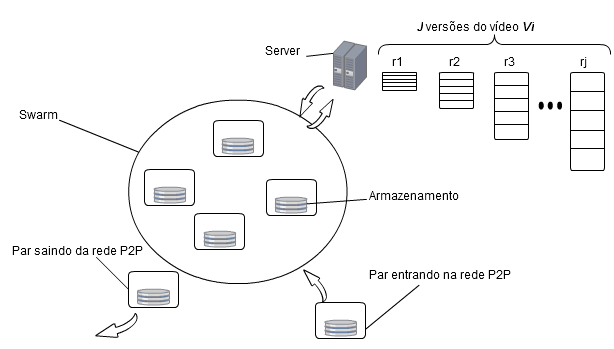
\includegraphics{figuras/Jversoes.png}
	%\label{figura1:Streaming adaptativo em uma rede P2P}
  \source{Autor, 2016}
\end{figure}




\section{Modelo de Otimização}

Na distribuição de vídeo em uma comunidade sem streaming adaptativo, o número de cópias de qualquer objeto é um inteiro a qualquer momento. Seja $x_{iv}$ uma variável zero-um a qual é igual a 1 se o par $i$ contém uma cópia do vídeo $v$ e 0 caso contrário.
Dado: $S_i$= ser a capacidade em bytes de armazenamento do par $i$ e  $S$=capacidade total de armazenamento da comunidade, tem-se:
\begin{equation}
S=\sum_{i=1}^{I}Si,\forall i\in I
\end{equation}
%\begin{equation}
% \forall i\in I
% \end{equation}
% \begin{equation}


	%\label{eq:equacao-exemplo1}



% \begin{equation}
%   Phit=1 -{v}q_{v}\prod_{i=1}^{I}(1-p_{i})^{x_{iv}}
% 	\label{eq:equacao-exemplo2}
% \end{equation}
Dado que $n_v$ é o número de réplicas do vídeo v, busca-se maximizar o número de cópias do vídeo:
\begin{equation}
%numero de copias do video v no swarm
n_{v}=\sum_{i=1}^{I}x_{iv}
	\label{eq:equacao-exemplo1}
\end{equation}
Sujeito a:

\begin{equation}
  \sum_{i=1}^{I}L_{v}x_{iv}\leq S, \forall i\in I
	\label{eq:equacao-exemplo3}
\end{equation}

\newcommand{\veth}{$h_{j}=(h_{1j},h_{2j},h_{3j},\ldots,H_j)$}
Porém, removida a restrição de integralidade, é possível desenvolver uma metodologia para determinar um limite superior na distribuição de conteúdo por meio do streaming adaptativo.
Adotamos que o vídeo $v$ é dividido em $J$ versões e cada versão é dividida em $H$ segmentos e que determinado $M$ de segmentos são necessários para reconstruir o vídeo. O tamanho de cada segmento $l$ é determinado por $l$=$L_j$/$M$, onde $L_j$ é o tamanho do vídeo na versão $j$.
Sobre esta análise, assumisse que os pares estão ativos na comunidade com probabilidade homogênea, $p_i=p$ para todos os pares.
Nos referimos ao h-ésimo segmento da versão $j$ como \veth. Para uma atribuição fixa de cópias aos pares. Dado $B_h$ ser o tamanho em bytes das réplicas dos $h_j$ segmentos armazenados na comunidade, Temos:

% Dado $n_{hj}$ ser o número de réplicas do segmento $h_j$ armazenados na comunidade e $B_h$ ser o tamanho em bytes de  $n_{hj}$, Temos:
\begin{equation}
Max  \ \ Bh=\sum_{j=1}^{J}\sum_{h=1}^{H}l_{jh}
\end{equation}\newline
$\forall j \in J$, $\forall h \in H.$
\newline
Sujeito \ a:
\begin{equation}
\sum_{i=1}^{I}\sum_{j=1}^{J}\sum_{h=1}^{H}x_{ijh}l_{jh} \leq S ,\ \forall i \in I
\end{equation}
\begin{equation}
\sum_{i=1}^{I}\sum_{j=1}^{J}x_{ijh} \leq 1 ,\ h = 1, \dots, H
\end{equation}

\begin{equation}
\sum_{j=1}^J\sum_{h=1}^{H}x_{ijh}\frac{l_{jh}}{U_i} \leq W ,i = 1, \dots, I
\end{equation}

A latência X dos m segmentos é menor ou igual ao tamanho da janela de tempo W.
\begin{equation}
X_m \leq W
\end{equation}
% \begin{equation}
%   \sum_{j=1}^{J}\sum_{h=1}^{H}\frac{Lj}{M}n_{jh}\leq S
% 	\label{eq:equacao-exemplo4}
% \end{equation}


\subsection{Streaming adaptativo}

No streaming adaptativo cada arquivo de vídeo é dividido em J versões e cada versão é dividida em H segmentos e todas as versões tem o mesmo tempo de playback X (Tian et al., 2013), Chama-se representação o conjunto de características do versionamento de um vídeo, tais como, o número de versões, a quantidade, tamanho e duração dos segmentos.


\begin{figure}[H]% H manda colocar exatamente nessa posição no texto (relativa aos parágrafos anterior e posterior)
	\centering
 	  \caption{Representação de um vídeo para streaming adaptativo}
		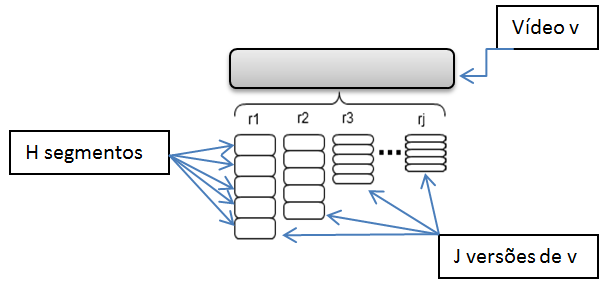
\includegraphics{figuras/segmentos.png}
	%\label{figura1:Streaming adaptativo em uma rede P2P}
  \source{Autor, 2016}
\end{figure}

O tracker identifica e mantem uma lista dos pares e seus recursos que entram no swarm, como banda de upload/download e capacidade de buffer, então fornece uma lista de pares possíveis para conexão, o qual, é capaz de consumir e compartilhar segmentos de vídeo.
Número de versões ideal (Xu et al., 2013)
Para escalonamento de download dos segmentos, um par usa políticas tais como oldest-first,rared first, the nearest-deadline-first,entre outras(Zhou:2011), entretanto, pretende-se usar uma política greedy e suas variações( priorizando segmentos com maior qualidade em termos de bits recebidos).



\section{Políticas de escalonamento para downloads de segmentos.}

Nosso objetivo é maximizar a quantidade de segmentos de maior qualidade entre os pares, para isso consideramos a taxa de bits, tamanho e duração do segmento, quanto ao par, consideramos a capacidade de armazenamento, banda de upload e download . Cada par mantém uma janela deslizante de tempo com segmentos para fazer o download, avançando a medida que o vídeo é reproduzido (Tian et al., 2013), portanto, é necessário escalonar dentro dessa janela de tempo, quais segmentos e suas respectivas taxas j do vídeo v serão baixados, de maneira que mantenha a maior qualidade, sem comprometer o fluxo de reprodução, a figura 2 ilustra esse cenário( construir a figura ).

\begin{figure}[H]% H manda colocar exatamente nessa posição no texto (relativa aos parágrafos anterior e posterior)
	\centering
 	  \caption{Problema de decisão sobre que segmentos e respectivas taxas j do vídeo v serão baixadas.}
		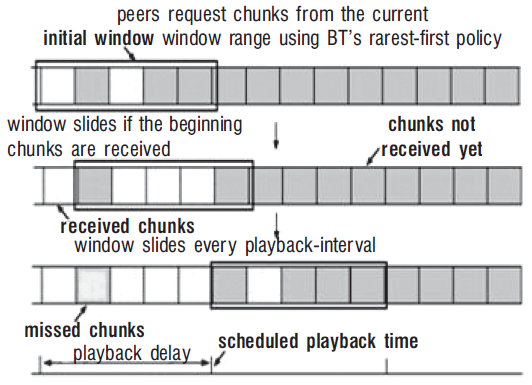
\includegraphics{figuras/janeladetempo.png}
	%\label{figura1:Streaming adaptativo em uma rede P2P}
  \source{Autor, 2016}
\end{figure}

Uma janela deslizante de tempo, é o intervalo de tempo W=bd/l, onde b é a taxa de visualização, d é a taxa de download e l é o tamanho do segmento, a taxa de download deve ser no mínimo igual a taxa de transmissão do objeto, para que o par tenha capacidade consumir a respectiva taxa produzida; esta janela possui os próximos h segmentos a serem baixados e avança a medida que estes são consumidos, segmentos que chegam após seu tempo de visualização podem ser descartados; além disso, evita-se baixar segmentos fora da janela de tempo, pois isso poderia degradar a continuidade do fluxo, uma vez que segmentos dentro da janela estão mais próximos de serem executados,  o problema desta restrição é a limitação do numero de segmentos que podem ser baixados e de uma tendência de download sequencial, em detrimento de outras politicas como por exemplo o rared-first utilizado no Bit-torrent, que prioriza o download de segmentos mais raros dentro do swarm.

Uma vez estabelecidas as representações de um vídeo com o número J de versões e de H segmentos, é necessário estabelecer políticas de escalonamento dentro da janela deslizante de tempo que busquem minimizar a carga sobre o servidor e maximizar os segmentos com maior qualidade em termos de bits recebidos dentro do swarm.

\chapter{Conclusão}

Texto de exemplo, texto de exemplo, texto de exemplo, texto de exemplo, texto de exemplo, texto de exemplo, texto de exemplo, texto de exemplo, texto de exemplo, texto de exemplo, texto de exemplo, texto de exemplo, texto de exemplo, texto de exemplo, texto de exemplo, texto de exemplo, texto de exemplo, texto de exemplo, texto de exemplo, texto de exemplo, texto de exemplo, texto de exemplo, texto de exemplo.

Texto de exemplo, texto de exemplo, texto de exemplo, texto de exemplo, texto de exemplo, texto de exemplo, texto de exemplo, texto de exemplo, texto de exemplo, texto de exemplo, texto de exemplo, texto de exemplo, texto de exemplo, texto de exemplo, texto de exemplo, texto de exemplo, texto de exemplo, texto de exemplo, texto de exemplo, texto de exemplo, texto de exemplo, texto de exemplo.

\section{Uma seção secundária}

Texto de exemplo, texto de exemplo, texto de exemplo, texto de exemplo, texto de exemplo, texto de exemplo, texto de exemplo, texto de exemplo, texto de exemplo, texto de exemplo, texto de exemplo, texto de exemplo, texto de exemplo, texto de exemplo, texto de exemplo, texto de exemplo, texto de exemplo, texto de exemplo, texto de exemplo, texto de exemplo, texto de exemplo, texto de exemplo, texto de exemplo.

Texto de exemplo, texto de exemplo, texto de exemplo, texto de exemplo, texto de exemplo, texto de exemplo, texto de exemplo, texto de exemplo, texto de exemplo, texto de exemplo, texto de exemplo, texto de exemplo, texto de exemplo, texto de exemplo, texto de exemplo, texto de exemplo, texto de exemplo, texto de exemplo, texto de exemplo, texto de exemplo, texto de exemplo, texto de exemplo, texto de exemplo.

\subsection{Uma seção terciária}

Texto de exemplo, texto de exemplo, texto de exemplo, texto de exemplo, texto de exemplo, texto de exemplo, texto de exemplo, texto de exemplo, texto de exemplo, texto de exemplo, texto de exemplo, texto de exemplo, texto de exemplo, texto de exemplo, texto de exemplo, texto de exemplo, texto de exemplo, texto de exemplo, texto de exemplo, texto de exemplo, texto de exemplo, texto de exemplo, texto de exemplo.

\subsection{Outra seção terciária}

Texto de exemplo, texto de exemplo, texto de exemplo, texto de exemplo, texto de exemplo, texto de exemplo, texto de exemplo, texto de exemplo, texto de exemplo, texto de exemplo, texto de exemplo, texto de exemplo, texto de exemplo, texto de exemplo, texto de exemplo, texto de exemplo, texto de exemplo, texto de exemplo, texto de exemplo, texto de exemplo, texto de exemplo, texto de exemplo, texto de exemplo.

\subsection{Mais uma seção terciária}

Texto de exemplo, texto de exemplo, texto de exemplo, texto de exemplo, texto de exemplo, texto de exemplo, texto de exemplo, texto de exemplo, texto de exemplo, texto de exemplo, texto de exemplo, texto de exemplo, texto de exemplo, texto de exemplo, texto de exemplo, texto de exemplo, texto de exemplo, texto de exemplo, texto de exemplo, texto de exemplo, texto de exemplo, texto de exemplo, texto de exemplo.

Texto de exemplo, texto de exemplo, texto de exemplo, texto de exemplo, texto de exemplo, texto de exemplo, texto de exemplo, texto de exemplo, texto de exemplo, texto de exemplo, texto de exemplo, texto de exemplo, texto de exemplo, texto de exemplo, texto de exemplo, texto de exemplo, texto de exemplo, texto de exemplo, texto de exemplo, texto de exemplo, texto de exemplo, texto de exemplo, texto de exemplo.

\section{Outra seção secundária}

Texto de exemplo, texto de exemplo, texto de exemplo, texto de exemplo, texto de exemplo, texto de exemplo, texto de exemplo, texto de exemplo, texto de exemplo, texto de exemplo, texto de exemplo, texto de exemplo, texto de exemplo, texto de exemplo, texto de exemplo, texto de exemplo, texto de exemplo, texto de exemplo, texto de exemplo, texto de exemplo, texto de exemplo, texto de exemplo, texto de exemplo.

Texto de exemplo, texto de exemplo, texto de exemplo, texto de exemplo, texto de exemplo, texto de exemplo, texto de exemplo, texto de exemplo, texto de exemplo, texto de exemplo, texto de exemplo, texto de exemplo, texto de exemplo, texto de exemplo, texto de exemplo, texto de exemplo, texto de exemplo, texto de exemplo, texto de exemplo, texto de exemplo, texto de exemplo, texto de exemplo, texto de exemplo.

Texto de exemplo, texto de exemplo, texto de exemplo, texto de exemplo, texto de exemplo, texto de exemplo, texto de exemplo, texto de exemplo, texto de exemplo, texto de exemplo, texto de exemplo, texto de exemplo, texto de exemplo, texto de exemplo, texto de exemplo, texto de exemplo, texto de exemplo, texto de exemplo, texto de exemplo, texto de exemplo, texto de exemplo, texto de exemplo, texto de exemplo.

\section{Mais uma seção secundária}

Texto de exemplo, texto de exemplo, texto de exemplo, texto de exemplo, texto de exemplo, texto de exemplo, texto de exemplo, texto de exemplo, texto de exemplo, texto de exemplo, texto de exemplo, texto de exemplo, texto de exemplo, texto de exemplo, texto de exemplo, texto de exemplo, texto de exemplo, texto de exemplo, texto de exemplo, texto de exemplo, texto de exemplo, texto de exemplo, texto de exemplo.

Texto de exemplo, texto de exemplo, texto de exemplo, texto de exemplo, texto de exemplo, texto de exemplo, texto de exemplo, texto de exemplo, texto de exemplo, texto de exemplo, texto de exemplo, texto de exemplo, texto de exemplo, texto de exemplo, texto de exemplo, texto de exemplo, texto de exemplo, texto de exemplo, texto de exemplo, texto de exemplo, texto de exemplo, texto de exemplo, texto de exemplo.

% ----------------------------------------------------------
% ELEMENTOS PÓS-TEXTUAIS
% ----------------------------------------------------------
\postextual
% ----------------------------------------------------------

% ----------------------------------------------------------
% Referências bibliográficas
% ----------------------------------------------------------
\bibliography{referencias}

% ----------------------------------------------------------
% Glossário
% ----------------------------------------------------------
%
% Consulte o manual da classe abntex2 para orientações sobre o glossário.
%
%\glossary

% ----------------------------------------------------------
% Apêndices
% ----------------------------------------------------------

% ---
% Inicia os apêndices
% ---
\begin{apendicesenv}

% Imprime uma página indicando o início dos apêndices
%\partapendices

%-------------------------------------------------------------------------
% Comentário adicional do PPgSI - Informações sobre ``apêndice''
%
% Para todos os captions/(títulos) (de seções, subseções, tabelas, 
% ilustrações, etc):
%     - em maiúscula apenas a primeira letra da sentença (do título), 
%       exceto nomes próprios, geográficos, institucionais ou Programas ou
%       Projetos ou siglas, os quais podem ter letras em maiúscula também.
%
% Todas  as tabelas, ilustrações (figuras, quadros, gráficos, etc. ), 
% anexos, apêndices devem obrigatoriamente ser citados no texto.
%      - a citação deve vir sempre antes da primeira vez em que a tabela, 
%        ilustração, etc., aparecer pela primeira vez.
%
%-------------------------------------------------------------------------
\chapter{Exemplo de apêndice}

Texto de exemplo, texto de exemplo, texto de exemplo, texto de exemplo, texto de exemplo, texto de exemplo, texto de exemplo, texto de exemplo, texto de exemplo, texto de exemplo, texto de exemplo, texto de exemplo, texto de exemplo, texto de exemplo, texto de exemplo, texto de exemplo, texto de exemplo, texto de exemplo, texto de exemplo.

\section*{1 Exemplo de seção de apêndice não apresentada no sumário}

Texto de exemplo, texto de exemplo, texto de exemplo, texto de exemplo, texto de exemplo, texto de exemplo, texto de exemplo, texto de exemplo, texto de exemplo, texto de exemplo, texto de exemplo, texto de exemplo, texto de exemplo, texto de exemplo, texto de exemplo, texto de exemplo, texto de exemplo, texto de exemplo, texto de exemplo.

\subsection*{1.1 Exemplo de subseção de apêndice não apresentada no sumário}

Texto de exemplo, texto de exemplo, texto de exemplo, texto de exemplo, texto de exemplo, texto de exemplo, texto de exemplo, texto de exemplo, texto de exemplo, texto de exemplo, texto de exemplo, texto de exemplo, texto de exemplo, texto de exemplo, texto de exemplo, texto de exemplo, texto de exemplo, texto de exemplo, texto de exemplo.

\subsection*{1.2 Exemplo de subseção de apêndice não apresentada no sumário}

Texto de exemplo, texto de exemplo, texto de exemplo, texto de exemplo, texto de exemplo, texto de exemplo, texto de exemplo, texto de exemplo, texto de exemplo, texto de exemplo, texto de exemplo, texto de exemplo, texto de exemplo, texto de exemplo, texto de exemplo, texto de exemplo, texto de exemplo, texto de exemplo, texto de exemplo.

\subsection*{1.3 Exemplo de subseção de apêndice não apresentada no sumário}

Texto de exemplo, texto de exemplo, texto de exemplo, texto de exemplo, texto de exemplo, texto de exemplo, texto de exemplo, texto de exemplo, texto de exemplo, texto de exemplo, texto de exemplo, texto de exemplo, texto de exemplo, texto de exemplo, texto de exemplo, texto de exemplo, texto de exemplo, texto de exemplo, texto de exemplo.

\section*{2 Exemplo de seção de apêndice não apresentada no sumário}

Texto de exemplo, texto de exemplo, texto de exemplo, texto de exemplo, texto de exemplo, texto de exemplo, texto de exemplo, texto de exemplo, texto de exemplo, texto de exemplo, texto de exemplo, texto de exemplo, texto de exemplo, texto de exemplo, texto de exemplo, texto de exemplo, texto de exemplo, texto de exemplo, texto de exemplo.

\section*{3 Exemplo de seção de apêndice não apresentada no sumário}

Texto de exemplo, texto de exemplo, texto de exemplo, texto de exemplo, texto de exemplo, texto de exemplo, texto de exemplo, texto de exemplo, texto de exemplo, texto de exemplo, texto de exemplo, texto de exemplo, texto de exemplo, texto de exemplo, texto de exemplo, texto de exemplo, texto de exemplo, texto de exemplo, texto de exemplo.


\chapter{Exemplo de apêndice}

Texto de exemplo, texto de exemplo, texto de exemplo, texto de exemplo, texto de exemplo, texto de exemplo, texto de exemplo, texto de exemplo, texto de exemplo, texto de exemplo, texto de exemplo, texto de exemplo, texto de exemplo, texto de exemplo, texto de exemplo, texto de exemplo, texto de exemplo, texto de exemplo, texto de exemplo.

\section*{1 Exemplo de seção de apêndice não apresentada no sumário}

Texto de exemplo, texto de exemplo, texto de exemplo, texto de exemplo, texto de exemplo, texto de exemplo, texto de exemplo, texto de exemplo, texto de exemplo, texto de exemplo, texto de exemplo, texto de exemplo, texto de exemplo, texto de exemplo, texto de exemplo, texto de exemplo, texto de exemplo, texto de exemplo, texto de exemplo.

\subsection*{1.1 Exemplo de subseção de apêndice não apresentada no sumário}

Texto de exemplo, texto de exemplo, texto de exemplo, texto de exemplo, texto de exemplo, texto de exemplo, texto de exemplo, texto de exemplo, texto de exemplo, texto de exemplo, texto de exemplo, texto de exemplo, texto de exemplo, texto de exemplo, texto de exemplo, texto de exemplo, texto de exemplo, texto de exemplo, texto de exemplo.

\subsection*{1.2 Exemplo de subseção de apêndice não apresentada no sumário}

Texto de exemplo, texto de exemplo, texto de exemplo, texto de exemplo, texto de exemplo, texto de exemplo, texto de exemplo, texto de exemplo, texto de exemplo, texto de exemplo, texto de exemplo, texto de exemplo, texto de exemplo, texto de exemplo, texto de exemplo, texto de exemplo, texto de exemplo, texto de exemplo, texto de exemplo.

\subsection*{1.3 Exemplo de subseção de apêndice não apresentada no sumário}

Texto de exemplo, texto de exemplo, texto de exemplo, texto de exemplo, texto de exemplo, texto de exemplo, texto de exemplo, texto de exemplo, texto de exemplo, texto de exemplo, texto de exemplo, texto de exemplo, texto de exemplo, texto de exemplo, texto de exemplo, texto de exemplo, texto de exemplo, texto de exemplo, texto de exemplo.

\section*{2 Exemplo de seção de apêndice não apresentada no sumário}

Texto de exemplo, texto de exemplo, texto de exemplo, texto de exemplo, texto de exemplo, texto de exemplo, texto de exemplo, texto de exemplo, texto de exemplo, texto de exemplo, texto de exemplo, texto de exemplo, texto de exemplo, texto de exemplo, texto de exemplo, texto de exemplo, texto de exemplo, texto de exemplo, texto de exemplo.

\section*{3 Exemplo de seção de apêndice não apresentada no sumário}

Texto de exemplo, texto de exemplo, texto de exemplo, texto de exemplo, texto de exemplo, texto de exemplo, texto de exemplo, texto de exemplo, texto de exemplo, texto de exemplo, texto de exemplo, texto de exemplo, texto de exemplo, texto de exemplo, texto de exemplo, texto de exemplo, texto de exemplo, texto de exemplo, texto de exemplo.


\chapter{Exemplo de apêndice}

Texto de exemplo, texto de exemplo, texto de exemplo, texto de exemplo, texto de exemplo, texto de exemplo, texto de exemplo, texto de exemplo, texto de exemplo, texto de exemplo, texto de exemplo, texto de exemplo, texto de exemplo, texto de exemplo, texto de exemplo, texto de exemplo, texto de exemplo, texto de exemplo, texto de exemplo.

\section*{1 Exemplo de seção de apêndice não apresentada no sumário}

Texto de exemplo, texto de exemplo, texto de exemplo, texto de exemplo, texto de exemplo, texto de exemplo, texto de exemplo, texto de exemplo, texto de exemplo, texto de exemplo, texto de exemplo, texto de exemplo, texto de exemplo, texto de exemplo, texto de exemplo, texto de exemplo, texto de exemplo, texto de exemplo, texto de exemplo.

\subsection*{1.1 Exemplo de subseção de apêndice não apresentada no sumário}

Texto de exemplo, texto de exemplo, texto de exemplo, texto de exemplo, texto de exemplo, texto de exemplo, texto de exemplo, texto de exemplo, texto de exemplo, texto de exemplo, texto de exemplo, texto de exemplo, texto de exemplo, texto de exemplo, texto de exemplo, texto de exemplo, texto de exemplo, texto de exemplo, texto de exemplo.

\subsection*{1.2 Exemplo de subseção de apêndice não apresentada no sumário}

Texto de exemplo, texto de exemplo, texto de exemplo, texto de exemplo, texto de exemplo, texto de exemplo, texto de exemplo, texto de exemplo, texto de exemplo, texto de exemplo, texto de exemplo, texto de exemplo, texto de exemplo, texto de exemplo, texto de exemplo, texto de exemplo, texto de exemplo, texto de exemplo, texto de exemplo.

\subsection*{1.3 Exemplo de subseção de apêndice não apresentada no sumário}

Texto de exemplo, texto de exemplo, texto de exemplo, texto de exemplo, texto de exemplo, texto de exemplo, texto de exemplo, texto de exemplo, texto de exemplo, texto de exemplo, texto de exemplo, texto de exemplo, texto de exemplo, texto de exemplo, texto de exemplo, texto de exemplo, texto de exemplo, texto de exemplo, texto de exemplo.

\section*{2 Exemplo de seção de apêndice não apresentada no sumário}

Texto de exemplo, texto de exemplo, texto de exemplo, texto de exemplo, texto de exemplo, texto de exemplo, texto de exemplo, texto de exemplo, texto de exemplo, texto de exemplo, texto de exemplo, texto de exemplo, texto de exemplo, texto de exemplo, texto de exemplo, texto de exemplo, texto de exemplo, texto de exemplo, texto de exemplo.

\section*{3 Exemplo de seção de apêndice não apresentada no sumário}

Texto de exemplo, texto de exemplo, texto de exemplo, texto de exemplo, texto de exemplo, texto de exemplo, texto de exemplo, texto de exemplo, texto de exemplo, texto de exemplo, texto de exemplo, texto de exemplo, texto de exemplo, texto de exemplo, texto de exemplo, texto de exemplo, texto de exemplo, texto de exemplo, texto de exemplo.




\end{apendicesenv}
% ---


% ----------------------------------------------------------
% Anexos
% ----------------------------------------------------------

% ---
% Inicia os anexos
% ---
\begin{anexosenv}

% Imprime uma página indicando o início dos anexos
%\partanexos


%-------------------------------------------------------------------------
% Comentário adicional do PPgSI - Informações sobre ``anexo''
%
% Para todos os captions/(títulos) (de seções, subseções, tabelas, 
% ilustrações, etc):
%     - em maiúscula apenas a primeira letra da sentença (do título), 
%       exceto nomes próprios, geográficos, institucionais ou Programas ou
%       Projetos ou siglas, os quais podem ter letras em maiúscula também.
%
% Todas  as tabelas, ilustrações (figuras, quadros, gráficos, etc. ), 
% anexos, apêndices devem obrigatoriamente ser citados no texto.
%      - a citação deve vir sempre antes da primeira vez em que a tabela, 
%        ilustração, etc., aparecer pela primeira vez.
%
%-------------------------------------------------------------------------
\chapter{Resumo das normas}
\label{anexoA}

Considerando a dificuldade para formatar um texto acadêmico sem conhecimento básico do conteúdo da norma NBR 14724 ``Informação e documentação – Trabalhos acadêmicos – Apresentação'', este anexo apresenta um resumo de alguns conceitos dessa norma, conforme publicada em julho de 2011. Sugere-se a leitura completa da norma para garantir que seu documento seja completamente aderente à mesma. Em alguns casos específicos, este anexo apresenta alguns ajustes da norma especificamente para o PPgSI.

\section*{1 NBR 14724: estrutura e algumas descrições}

A estrutura de uma tese, dissertação ou qualquer outro trabalho acadêmico, deve compreender elementos pré-textuais, elementos textuais e elementos pós-textuais, que aparecem no texto na seguinte ordem:

\subsection*{1.1 Elementos pré-textuais}

\begin{itemize}
	\item Capa (obrigatório)
	\item	Folha de rosto (obrigatório)
	\item	Errata (opcional)
	\item	Folha de aprovação (obrigatório)
	\item	Dedicatória (opcional)
	\item	Agradecimentos (opcional)
	\item	Epígrafe (opcional)
	\item	Resumo em língua vernácula (obrigatório)
	\item	Resumo em língua estrangeira (obrigatório)
	\item	Listas de ilustrações: lista de figuras, lista de algoritmos, lista de quadros, etc. (opcional)
	\item	Lista de tabelas (opcional)
	\item	Lista de abreviaturas e siglas (opcional)
	\item	Lista de símbolos (opcional)
	\item	Sumário (obrigatório)
\end{itemize}

\subsection*{1.2 Elementos textuais}

\begin{itemize}
	\item	Introdução
	\item	Desenvolvimento
	\item	Conclusão
\end{itemize}

\subsection*{1.3 Elementos pós-textuais}

\begin{itemize}
	\item	Referências (obrigatório)
	\item	Apêndice (opcional)
	\item	Anexo (opcional)
	\item	Glossário (opcional)
\end{itemize}

\section*{2 Definições relacionadas a elementos pré-textuais}

A seguir, são apresentadas algumas definições contidas na norma relacionadas a elementos pré-textuais.

\subsection*{2.1 Capa}

Elemento obrigatório, para proteção externa e sobre o qual se imprimem informações que ajudam na identificação e uso do trabalho, na seguinte ordem:
\begin{enumerate}
	\item Nome completo do autor: responsável intelectual do trabalho.
	\item	Título principal do trabalho: deve ser claro e preciso, identificando o seu conteúdo e possibilitando a indexação e recuperação da informação.
	\item	Subtítulo (se houver): deve ser evidenciada sua subordinação ao título principal, precedido de dois pontos (:).
	\item	Número do volume (obrigatório apenas se houver mais de um volume, de forma que deve constar em cada capa a especificação do respectivo volume).
	\item	Local (cidade) da instituição de apresentação.
	\item	Ano do depósito (entrega).
\end{enumerate}

\subsection*{2.2 Folha de rosto (anverso)}

Os elementos do anverso da folha de rosto devem figurar na seguinte ordem:
\begin{enumerate}
	\item	Nome completo do autor: responsável intelectual do trabalho.
	\item	Título principal do trabalho: deve ser claro e preciso, identificando o seu conteúdo e possibilitando a indexação e recuperação da informação.
	\item	Subtítulo (se houver): deve ser evidenciada sua subordinação ao título principal, precedido de dois pontos (:).
	\item	Número do volume (obrigatório apenas se houver mais de um volume, de forma que deve constar em cada capa a especificação do respectivo volume).
	\item	Natureza (tese, dissertação e outros) e objetivo (aprovação em disciplina, grau pretendido e outros); nome da instituição a que é submetido; área de concentração.
	\item	Nome do orientador e, se houver, do co-orientador.
	\item	Local (cidade) da instituição de apresentação.
	\item	Ano de depósito (entrega).
\end{enumerate}

\subsection*{2.3 Folha de rosto (verso)}

No verso da folha de rosto deve constar a ficha catalográfica, conforme o Código de Catalogação Anglo-Americano – CCAA2.

\subsection*{2.4 Folha de aprovação}

Elemento obrigatório, que contém autor, título por extenso e subtítulo, se houver, local e data de aprovação, nome e instituição dos membros componentes da banca examinadora.

\subsection*{2.5 Dedicatória e agradecimentos}

Elementos opcionais. Os agradecimentos devem ser dirigidos apenas àqueles que contribuíram de maneira relevante à elaboração do trabalho.

\subsection*{2.6 Resumo na língua vernácula}

Elemento obrigatório, que consiste na apresentação concisa dos pontos relevantes de um texto; constitui-se em uma sequência de frases concisas e objetivas, e não de uma simples enumeração de tópicos, não ultrapassando 500 palavras, seguido, logo abaixo, das palavras representativas do conteúdo do trabalho, isto é, palavras-chave e/ou descritores.

\subsection*{2.7 Resumo em língua estrangeira}

Elemento obrigatório, que consiste em uma versão do resumo em idioma de divulgação internacional (em inglês Abstract, em castelhano Resumen, em francês Résumé, por exemplo). Deve ser seguido das palavras representativas do conteúdo do trabalho, isto é, palavras-chave e/ou descritores, na respectiva língua estrangeira.

\subsection*{2.8 Lista de figuras e lista de tabelas}

Elementos opcionais, elaborados de acordo com a ordem apresentada no texto, com cada item acompanhado do respectivo número da página.

\subsection*{2.9 Lista de abreviaturas e siglas}

Elemento opcional. Consiste na relação alfabética das abreviaturas e siglas usadas no texto, seguidas das palavras ou expressões correspondentes grafadas por extenso.

\subsection*{2.10 Lista de símbolos}

Elemento opcional, elaborado de acordo com a ordem apresentada no texto, com o devido significado.

\subsection*{2.11 Sumário}

Elemento obrigatório, que consiste na enumeração das principais divisões (seções e outras partes do trabalho) dos elementos textuais e pós-textuais, na mesma ordem e grafia em que a matéria nele sucede, acompanhado do respectivo número da página.

\section*{3 Definições relacionadas a elementos textuais}

O autor deve criar quantas seções primárias (também chamadas informalmente de capítulos) desejar para tratar dos seguintes elementos textuais que são obrigatórios: introdução, desenvolvimento e conclusão. Normalmente, existe apenas uma seção primária para a introdução, uma ou mais seções primárias para o desenvolvimento, e apenas uma seção primária para a conclusão.

\section*{4 Definições relacionadas a elementos pós-textuais}

A seguir, são apresentadas algumas definições contidas na norma relacionadas a elementos pós-textuais.

\subsection*{4.1 Apêndice}

Elemento opcional, que consiste em um texto ou documento elaborado pelo próprio autor, a fim de complementar sua argumentação, sem prejuízo da unidade nuclear do trabalho. Um apêndice deve ser identificado por uma letra maiúscula, seguida por um hífen (entre caracteres de espaço), seguido pelo respectivo título. Os apêndices devem ser identificados por letras consecutivas, a partir da letra ``A'' (independentemente dos anexos).

\subsection*{4.2 Anexo}

Elemento opcional, que consiste em um texto ou documento não elaborado pelo autor, a fim de fundamentar, comprovar ou ilustrar a argumentação do autor. Um anexo deve ser identificado por uma letra maiúscula, seguida por um hífen (entre caracteres de espaço), seguido pelo respectivo título. Os anexos devem ser identificados por letras consecutivas, a partir da letra ``A'' (independentemente dos apêndices).

\subsection*{4.3 Glossário}

Elemento opcional, que consiste em uma lista em ordem alfabética de palavras ou de expressões técnicas de uso restrito ou de sentido obscuro, usadas no texto, acompanhadas das respectivas definições.

\section*{5 Formas de apresentação}

A seguir, são apresentadas algumas definições contidas na norma relacionadas a formas de apresentação em geral.

\subsection*{5.1 Formato}

O texto deve estar impresso em papel branco, formato A4 (21,0 cm 29,7 cm), apenas no anverso da folha (ou seja, na ``frente'' da folha), excetuando-se a folha de rosto que deve estar impressa tanto no anverso quanto no verso (com a ficha catalográfica).

\subsection*{5.2 Projeto gráfico}

O projeto gráfico é de responsabilidade do autor.

\subsection*{5.3 Fonte}


Usar sempre cor preta.

Usar sempre tamanho de fonte 12, com as seguintes exceções: tamanho de fonte 10 para citações longas (com mais de três linhas), notas de rodapé, legendas de ilustração e de tabela, fontes de ilustração e de tabela, números de página; e tamanho de fonte maiores para títulos de seção (conforme apresentado na seção 6.1 a seguir).

\subsection*{5.4 Margens}

Todas as folhas devem apresentar margens esquerda e superior de 3 cm; e margens direita e inferior de 2 cm, considerando impressão apenas no anverso (ou seja, apenas na ``frente''). 

Se a impressão precisar, por algumo motivo especial, ser realizada em anverso e verso (ou seja, em frente e verso), neste caso, há que se configurar as margens de forma diferente, conforme detalhes da norma ABNT, além de outros detalhes de configuração; por isso solicita-se não realizar impressão em frente e verso.

\subsection*{5.5 Espaçamento entre linhas}

Usar sempre espaçamento entre linhas de 1,5 linhas, com as seguintes exceções: espaçamento entre linhas ``simples'' para citações longas (com mais de três linhas), notas de rodapé, referências, resumos (em vernáculo e em língua estrangeira), legendas de ilustração e de tabela, fontes de ilustração e de tabela, ficha catalográfica, natureza do trabalho, grau pretendido, nome da instituição a que é submetido, e área de concentração; e espaçamento entre linhas ``duplo'' para equações e fórmulas e para separação das referências entre si.

Os títulos das seções devem começar na margem superior da folha separados do texto que os sucede por um espaço em branco de 1,5 e, da mesma forma, os títulos das subseções devem ser separados do texto que os precede, ou que os sucede, por um espaço em branco de 1,5.

\subsection*{5.6 Numeração das seções}

O indicativo numérico de uma seção precede seu título, alinhado à esquerda, separado por um espaço de caractere. Nos títulos sem indicativo numérico, como lista de ilustrações, sumário, resumo, referências e outros, devem ser centralizados.

Para evidenciar a sistematização do conteúdo do trabalho, deve-se adotar a numeração progressiva para as seções do texto. Os títulos das seções primárias (chamadas informalmente de capítulos), por serem as principais divisões do texto, devem iniciar em folha distinta. Títulos das seções e subseções devem ser destacados gradativamente, usando-se os recursos de negrito, itálico ou grifo e redondo, caixa alta ou versal.

\subsection*{5.7 Paginação}

Todas as folhas do trabalho, a partir da folha de rosto (desconsiderando a capa, mas considerando a ficha catalográfica), devem ser contadas sequencialmente, mas não numeradas. A numeração é colocada, a partir da primeira folha da dos elementos textuais (ou seja, a partir da ``Introdução''), em algarismos arábicos, no canto superior direito da folha, a 2 cm da borda superior, ficando o último algarismo a 2 cm da borda direita da folha.

Havendo apêndices e/ou anexos, suas folhas devem ser numeradas de maneira contínua e sua paginação deve dar seguimento à do texto principal, em algarismos arábicos.

No caso de o trabalho ser constituído de mais de um volume, deve-se manter uma única sequência de numeração das folhas, do primeiro ao último volume.

\subsection*{5.8 Equações e fórmulas}

Equações e fórmulas devem aparecer destacadas no texto, para facilitar sua leitura. 

Se as equações e fórmulas forem apresentadas na sequência normal do texto (ou seja, dentro do próprio parágrafo normal de texto), é permitido usar um espaçamento entre linhas duplo para comportar seus elementos (ou seja, expoentes, índices e outros). 

Se as equações e fórmulas forem apresentadas fora do parágrafo, então elas devem ser centralizadas e, se necessário, devem ser numeradas. Quando fragmentadas em mais de uma linha, por falta de espaço, devem ser interrompidas antes do sinal de igualdade ou depois dos sinais de adição, subtração, multiplicação e divisão.

\subsection*{5.9 Ilustrações}

Cada tipo de ilustração (tais como figura, gráfico, algoritmo, fotografia, quadro, esquema, desenhos, esquemas, fluxogramas, mapa, organograma, planta, retrato, entre outros) tem numeração independente e consecutiva. 

Inserir a ilustração o mais próximo possível do parágrafo em que ela é citada pela primeira vez no texto; nunca inserir uma ilustração antes de ela ser citada pela primeira vez no texto. Toda ilustração inserida no trabalho deve ser citada pelo menos uma vez no texto.

Qualquer que seja o tipo da ilustração, ela deve obrigatoriamente ter uma identificação (ou seja, um título), que deve aparecer sempre na parte superior da ilustração, precedida pela palavra que identifica seu tipo, por exemplo ``Figura'', seguida de seu número de ordem de ocorrência no texto em algarismo arábico, e de um hífen entre caracteres de espaço (`` – ''), em fonte com tamanho 12, sem negrito, sem itálico, com apenas a primeira letra da sentença maiúscula, sem ponto final, e em espaçamento simples. Exemplo: ``Figura 1 – Título da ilustração''.

Para toda ilustração, deve ser apresentada também obrigatoriamente sua fonte (mesmo quando a fonte é o próprio autor do trabalho). A fonte deve apresentada na parte inferior da ilustração e ser informada no seguinte formato: palavra ``Fonte'', seguida pelo caractere dois pontos ``:'', seguido por um caractere de espaço, seguido pela citação de onde a ilustração foi obtida (conforme regras de citação da norma ABNT) ou seguido pelo nome completo do autor do trabalho, por uma vírgula e pelo ano de elaboração do trabalho (caso a ilustração seja de elaboração do próprio autor), em fonte com tamanho 10, sem negrito, sem itálico, sem ponto final, e em espaçamento simples. Exemplo 1 (quando se trata de fonte externa): ``Fonte: citação conforme norma ABNT''; Exemplo 2 (quando se trata do próprio autor do trabalho): ``Fonte: Nome Completo, Ano''.

Para referenciar uma ilustração (por exemplo, do tipo ``figura'') no texto, há duas formas: \textit{(i)} se a referência à figura fizer parte do texto, mesmo que dentro de parênteses, use a palavra ``figura'' com todas as letras em minúsculo, por exemplo – ``A figura 5 apresenta um exemplo de (...)'' ou ``(...) esses dados já foram apresentados na seção anterior (ver figura 5)''; \textit{(ii)} se a referência à figura estiver completamente isolada do texto, dentro de parênteses, use a palavra ``Figura'' com a inicial em maiúsculo, por exemplo ``(...) para um entendimento mais claro, essas informações estão apresentadas graficamente (Figura 5)''.

\subsection*{5.10 Tabelas}

As tabelas têm numeração independente e consecutiva das ilustrações.

Inserir a tabela o mais próximo possível do parágrafo em que ela é citada pela primeira vez no texto; nunca inserir uma tabela antes de ela ser citada pela primeira vez no texto. Toda tabela inserida no trabalho deve ser citada pelo menos uma vez no texto.

Toda tabela deve obrigatoriamente ter uma identificação (ou seja, um título), que deve aparece na parte superior, precedida pela palavra ``Tabela'', seguida de seu número de ordem de ocorrência no texto em algarismo arábico, e de um hífen entre caracteres de espaço (`` – ''), em fonte com tamanho 12, sem negrito, sem itálico, com apenas a primeira letra da sentença maiúscula, sem ponto final, e em espaçamento simples. Exemplo: ``Tabela 1 – Título da tabela''.

Para toda tabela, deve ser apresentada também obrigatoriamente sua fonte (mesmo quando a fonte é o próprio autor do trabalho). A fonte deve apresentada na parte inferior da tabela e ser informada no seguinte formato: palavra ``Fonte'', seguida pelo caractere dois pontos ``:'', seguido por um caractere de espaço, seguido pela citação de onde a fonte foi obtida (conforme regras de citação da norma ABNT) ou seguido pelo nome completo do autor do trabalho, por uma vírgula e pelo ano de elaboração do trabalho (caso a fonte seja de elaboração do próprio autor), em fonte com tamanho 10, sem negrito, sem itálico, sem ponto final, e em espaçamento simples. Exemplo 1 (quando se trata de fonte externa): ``Fonte: citação conforme norma ABNT''; Exemplo 2 (quando se trata do próprio autor do trabalho): ``Fonte: Nome Completo, Ano''.

Usar traços horizontais apenas para delimitar o cabeçalho da tabela e o início e o fim da tabela. Não usar traços horizontais para separar cada linha de conteúdo da tabela e também não usar traços verticais para separar cada coluna de conteúdo da tabela. 

Se a tabela não couber em uma folha, ela deve ser continuada nas folhas seguintes. Nesse caso, a tabela não deve ser delimitada por traço horizontal na parte inferior nas primeiras folhas (mas sim apenas na última folha em que ela realmente é finalizada), e a legenda e o cabeçalho da tabela devem ser repetidos nas folhas seguintes. Além disso, as folhas devem ter as seguintes indicações: ``continua'' (no fim das primeiras folhas); ``continuação'' (no início das folhas intermediárias, se houver) e ``conclusão'' (no início da última folha).

Para referenciar uma tabela no texto, há duas formas: \textit{(i)} se a referência à tabela fizer parte do texto, mesmo que dentro de parênteses, use a palavra ``tabela'' com todas as letras em minúsculo, por exemplo – ``A tabela 5 apresenta um exemplo de (...)'' ou ``(...) esses dados já foram apresentados na seção anterior (ver tabela 5)''; \textit{(ii)} se a referência à tabela estiver completamente isolada do texto, dentro de parênteses, use a palavra ``Tabela'' com a inicial em maiúsculo, por exemplo ``(...) para um entendimento mais claro, essas informações estão apresentadas graficamente (Tabela 5)''.

Não confundir ``tabela'' com ``quadro''. Uma tabela deve ter dados numéricos como informação central. Outros tipos de organização de informações devem ser apresentados em quadros, que é um dos tipos de ilustração. A formatação de um quadro é muito parecida a de uma tabela, porém todos os traços horizontais e verticais devem ser apresentados.

\section*{6 Outras normas}

\subsection*{6.1 Seções}

As seções primárias são as principais divisões do texto, denominadas informalmente de ``capítulos''. As seções primárias podem ser divididas em seções secundárias; as secundárias em terciárias, e assim por diante, até a quinta ordem, em formatação distinta. Não é possível dividir o texto mais do que a quinta ordem.

A formatação adotada para este \textit{template} em particular é a seguinte:

\begin{itemize}
	\item Seções primárias: tamanho 16, com negrito.
	\item Seções secundárias: tamanho 15, com negrito.
	\item Seções terciárias: tamanho 14, com negrito.
	\item Seções quartenárias: tamanho 13, sem negrito.
	\item Seções quinárias: tamanho 12, sem negrito.
\end{itemize}

São empregados algarismos arábicos na numeração. O ``indicativo'' de uma seção precede o título ou a primeira palavra do texto, se não houver título, separado por um espaço. O indicativo da seção secundária é constituído pelo indicativo da seção primária que a precede seguido do número que lhe foi atribuído na sequência do assunto e separado por ponto. Repete-se o mesmo processo em relação às demais seções. Na leitura, não se lê os pontos (por exemplo: ``2.1.1'' lê-se ``dois um um'').

Os indicativos devem ser citados no texto de acordo com os seguintes exemplos: (...) na seção 4 (...); (...) no capítulo 2 (...); (...) ver 9.2 (...); (...) em 1.1.2.2 parág. 3º [ou] (...) no 3º parágrafo de 1.1.2.2; (...) (Seção 2.1) (...).

\subsection*{6.2 Referências bibliográficas e citações às referências bibliográficas}

A norma é bastante complexa e extensa em relação às regras de referências bibliográficas (cerca de 19 páginas) e citações às referências bibliográficas, não sendo possível fazer um resumo aqui. Assim, é necessário fazer uma consulta às normas detalhadas.

As referências devem ser apresentadas em ordem alfabética, com as citações no texto obedecendo ao sistema autor-data.Todos os documentos relacionados nas Referências devem ser citados no texto, assim como todas as citações do texto devem constar nas Referências.

\chapter{Exemplo de anexo}

Texto de exemplo, texto de exemplo, texto de exemplo, texto de exemplo, texto de exemplo, texto de exemplo, texto de exemplo, texto de exemplo, texto de exemplo, texto de exemplo, texto de exemplo, texto de exemplo, texto de exemplo, texto de exemplo, texto de exemplo, texto de exemplo, texto de exemplo, texto de exemplo, texto de exemplo.

\section*{1 Exemplo de seção de anexo não apresentada no sumário}

Texto de exemplo, texto de exemplo, texto de exemplo, texto de exemplo, texto de exemplo, texto de exemplo, texto de exemplo, texto de exemplo, texto de exemplo, texto de exemplo, texto de exemplo, texto de exemplo, texto de exemplo, texto de exemplo, texto de exemplo, texto de exemplo, texto de exemplo, texto de exemplo, texto de exemplo.

\subsection*{1.1 Exemplo de subseção de anexo não apresentada no sumário}

Texto de exemplo, texto de exemplo, texto de exemplo, texto de exemplo, texto de exemplo, texto de exemplo, texto de exemplo, texto de exemplo, texto de exemplo, texto de exemplo, texto de exemplo, texto de exemplo, texto de exemplo, texto de exemplo, texto de exemplo, texto de exemplo, texto de exemplo, texto de exemplo, texto de exemplo.

\subsection*{1.2 Exemplo de subseção de anexo não apresentada no sumário}

Texto de exemplo, texto de exemplo, texto de exemplo, texto de exemplo, texto de exemplo, texto de exemplo, texto de exemplo, texto de exemplo, texto de exemplo, texto de exemplo, texto de exemplo, texto de exemplo, texto de exemplo, texto de exemplo, texto de exemplo, texto de exemplo, texto de exemplo, texto de exemplo, texto de exemplo.

\subsection*{1.3 Exemplo de subseção de anexo não apresentada no sumário}

Texto de exemplo, texto de exemplo, texto de exemplo, texto de exemplo, texto de exemplo, texto de exemplo, texto de exemplo, texto de exemplo, texto de exemplo, texto de exemplo, texto de exemplo, texto de exemplo, texto de exemplo, texto de exemplo, texto de exemplo, texto de exemplo, texto de exemplo, texto de exemplo, texto de exemplo.

\section*{2 Exemplo de seção de anexo não apresentada no sumário}

Texto de exemplo, texto de exemplo, texto de exemplo, texto de exemplo, texto de exemplo, texto de exemplo, texto de exemplo, texto de exemplo, texto de exemplo, texto de exemplo, texto de exemplo, texto de exemplo, texto de exemplo, texto de exemplo, texto de exemplo, texto de exemplo, texto de exemplo, texto de exemplo, texto de exemplo.

\section*{3 Exemplo de seção de anexo não apresentada no sumário}

Texto de exemplo, texto de exemplo, texto de exemplo, texto de exemplo, texto de exemplo, texto de exemplo, texto de exemplo, texto de exemplo, texto de exemplo, texto de exemplo, texto de exemplo, texto de exemplo, texto de exemplo, texto de exemplo, texto de exemplo, texto de exemplo, texto de exemplo, texto de exemplo, texto de exemplo.

\chapter{Exemplo de anexo}

Texto de exemplo, texto de exemplo, texto de exemplo, texto de exemplo, texto de exemplo, texto de exemplo, texto de exemplo, texto de exemplo, texto de exemplo, texto de exemplo, texto de exemplo, texto de exemplo, texto de exemplo, texto de exemplo, texto de exemplo, texto de exemplo, texto de exemplo, texto de exemplo, texto de exemplo.

\section*{1 Exemplo de seção de anexo não apresentada no sumário}

Texto de exemplo, texto de exemplo, texto de exemplo, texto de exemplo, texto de exemplo, texto de exemplo, texto de exemplo, texto de exemplo, texto de exemplo, texto de exemplo, texto de exemplo, texto de exemplo, texto de exemplo, texto de exemplo, texto de exemplo, texto de exemplo, texto de exemplo, texto de exemplo, texto de exemplo.

\subsection*{1.1 Exemplo de subseção de anexo não apresentada no sumário}

Texto de exemplo, texto de exemplo, texto de exemplo, texto de exemplo, texto de exemplo, texto de exemplo, texto de exemplo, texto de exemplo, texto de exemplo, texto de exemplo, texto de exemplo, texto de exemplo, texto de exemplo, texto de exemplo, texto de exemplo, texto de exemplo, texto de exemplo, texto de exemplo, texto de exemplo.

\subsection*{1.2 Exemplo de subseção de anexo não apresentada no sumário}

Texto de exemplo, texto de exemplo, texto de exemplo, texto de exemplo, texto de exemplo, texto de exemplo, texto de exemplo, texto de exemplo, texto de exemplo, texto de exemplo, texto de exemplo, texto de exemplo, texto de exemplo, texto de exemplo, texto de exemplo, texto de exemplo, texto de exemplo, texto de exemplo, texto de exemplo.

\subsection*{1.3 Exemplo de subseção de anexo não apresentada no sumário}

Texto de exemplo, texto de exemplo, texto de exemplo, texto de exemplo, texto de exemplo, texto de exemplo, texto de exemplo, texto de exemplo, texto de exemplo, texto de exemplo, texto de exemplo, texto de exemplo, texto de exemplo, texto de exemplo, texto de exemplo, texto de exemplo, texto de exemplo, texto de exemplo, texto de exemplo.

\section*{2 Exemplo de seção de anexo não apresentada no sumário}

Texto de exemplo, texto de exemplo, texto de exemplo, texto de exemplo, texto de exemplo, texto de exemplo, texto de exemplo, texto de exemplo, texto de exemplo, texto de exemplo, texto de exemplo, texto de exemplo, texto de exemplo, texto de exemplo, texto de exemplo, texto de exemplo, texto de exemplo, texto de exemplo, texto de exemplo.

\section*{3 Exemplo de seção de anexo não apresentada no sumário}

Texto de exemplo, texto de exemplo, texto de exemplo, texto de exemplo, texto de exemplo, texto de exemplo, texto de exemplo, texto de exemplo, texto de exemplo, texto de exemplo, texto de exemplo, texto de exemplo, texto de exemplo, texto de exemplo, texto de exemplo, texto de exemplo, texto de exemplo, texto de exemplo, texto de exemplo.

\end{anexosenv}

%---------------------------------------------------------------------
% INDICE REMISSIVO
%---------------------------------------------------------------------
%%%%%MF\phantompart
%%%%%MF\printindex
%---------------------------------------------------------------------

\end{document}
